% !TeX document-id = {236dae5e-e9c5-4be7-838f-9dddbf9d2537}
% !TEX program = XeLaTeX
%\documentclass{cumcmthesis}
\documentclass[withoutpreface,bwprint,fontset=macnew]{cumcmthesis} %去掉封面与编号页,电子版提交的时候使用。


\usepackage[framemethod=TikZ]{mdframed}
\usepackage{url}   % 网页链接
\usepackage{subcaption} % 子标题
\title{``FAST"主动反射面的形状调节}

\begin{document}
	
	
	\maketitle
	\begin{abstract}
		本文主要研究如何在限制主索网节点径向移动范围、主索网节点相邻点间距变化范围、指定理想抛物面焦点的情况下,求解出最优理想抛物面,使得主索网节点能够尽可能逼近该理想抛物面,从而最大化馈源舱接收比。

		对于问题一,由于理想抛物面的对称轴与焦点已经确定,我们用焦准距作为确定理想抛物面的唯一参数。在不同的焦准距下,理想抛物面的位置不同,主动反射面对理想抛物面的拟合程度也不同。我们建立了一个\textbf{双层优化}模型,外层以主动反射面和理想抛物面的拟合程度为最小化目标,求解最优的焦准距;内层在给定某一特定理想抛物面的情形下,定义各主索网节点与理想抛物面间距离,建立以最小化距离平方和为优化目标、以促动器移动限制和主索长度变化限制为约束条件的非线性规划模型。对于外层优化模型,由于只有一个决策变量,我们采用变步长枚举法求解,并发现其具有很好的凸性;对于内层优化模型,它是一个具有复杂条件的高维非线性规划问题,我们提供了两种求解思路:一是对节点进行\textbf{分组优化},对具有相同位置特征的节点进行统一处理,从而大大减少维数;二是将约束条件进行简化,得到具有唯一最优解的\textbf{凸二次规划}形式。实验结果证明凸二次规划模型对理想抛物面拟合程度更高、接收比更高,故最后确定理想抛物面的方程为
		$
		x^2 + y^2 -561.53494z - 168908.213082 = 0
		$
		
		对于问题二,我们采用\textbf{基坐标变换},将入射光线以及各主索网节点位置坐标变换到以光线入射反方向为 z 轴方向的坐标系中,该变换能够保证空间相对位置不发生改变。随后采用第一问的凸二次规划模型求解出各主索网节点在新坐标系之中的位置坐标、促动器伸缩量。最后将位置坐标逆变换至初始坐标系,得出结果。得到理想抛物面的顶点坐标为 $(-49.38425683, -36.9374232, -294.4013909)$,其余结果请见附件4。

		对于问题三,我们综合考虑了面板倾斜角度,面板大小等因素,以信号的反射为基础建立了接收比计算模型。该模型用来描述面板将信号反射至馈源舱的物理过程,通过计算\textbf{馈源舱接收信号通量}与\textbf{工作抛物面整体信号通量}之比,得到馈源舱接收比。同时,我们通过理论分析求出在所有面板均能照射至馈源舱时的\textbf{接收比上限}为 $1.398\%$,不同情况下接收比如下表:
		\begin{table}[!htbp]
			\centering
			\begin{tabular}{cccc}
				\toprule[1.5pt]
				$ $ & 基准反射球面 & 求解后工作抛物面 & 理想抛物面接收比\\
				\midrule[1pt]
				接收比 & $0.861139\%$ & $1.137517\%$ & $1.175547\%$\\
				\bottomrule[1.5pt]
			\end{tabular}
		\end{table}

		最后,我们提出了模型的不足与改进,并分析了馈源舱吸收比与馈源舱半径的关系,具有一定的现实意义。
		
		\keywords{抛物面拟合\quad 最优化模型\quad 凸二次规划\quad 双层优化\quad 基坐标变换}
	\end{abstract}

	% \newpage
	
	\section{问题背景与重述}
	\subsection{问题背景}
	我国500M口径球面射电望远镜(Five-hundred-meter Aperture Spherical radio Telescope,简称 FAST)于2020年1月11日通过验收,正式投入使用。旨在观测宇宙中氢元素、脉冲星、星际分子等宇宙信号,进而推进在天文学以及物理学方面的研究。对于我国相关领域的发展及建设具有众大意义。是我国具有自主知识产权的目前世界上单口径最大、灵敏度最高的射电望远镜。

	作为一个大型系统性工程,FAST望远镜的落建过程中我国应用并研发了多种工程技术,如馈源舱信号接收技术、馈源舱控制技术、反射面结构调整技术等等。充分实践了我国的科学前沿重大原创突破要求、创新驱动发展战略。

	FAST由主动反射面系统(主索网、反射面板、下拉索、促动器)和信号接收系统(馈源舱)组成。口径500m、半径300.4m的球冠形索网是FAST反射面的主体支承结构。主索网通过主索节点与连接在促动器上的下拉索相连。通过促动器的主动伸缩,可以控制索网在基准态球面和工作态抛物面之间转换及主动变位。

	\subsection{问题重述}

	FAST的馈源舱在一个与索网基准态球面同心(球心C)、半径为$0.534R$的球面(焦面)上运动,其接收范围为直径1m的圆盘。

	在基准态球面时,促动器的伸缩量为0;促动器沿径向伸缩,范围为$-0.6 \textasciitilde +0.6$m(以趋向球心方向为正向)。与促动器连接的下拉索长度固定。

	观测天体S时,馈源舱中心移动到直线SC与焦面的交点P处,为使馈源舱接收到尽可能多的信号,通过促动器伸缩调整基准态球面的部分反射面板形成以SC为对称轴,P为焦点的旋转抛物面(工作态抛物面)。
	
	\begin{figure}[!h]
		\centering
		\begin{minipage}[c]{0.48\textwidth}
			\centering
			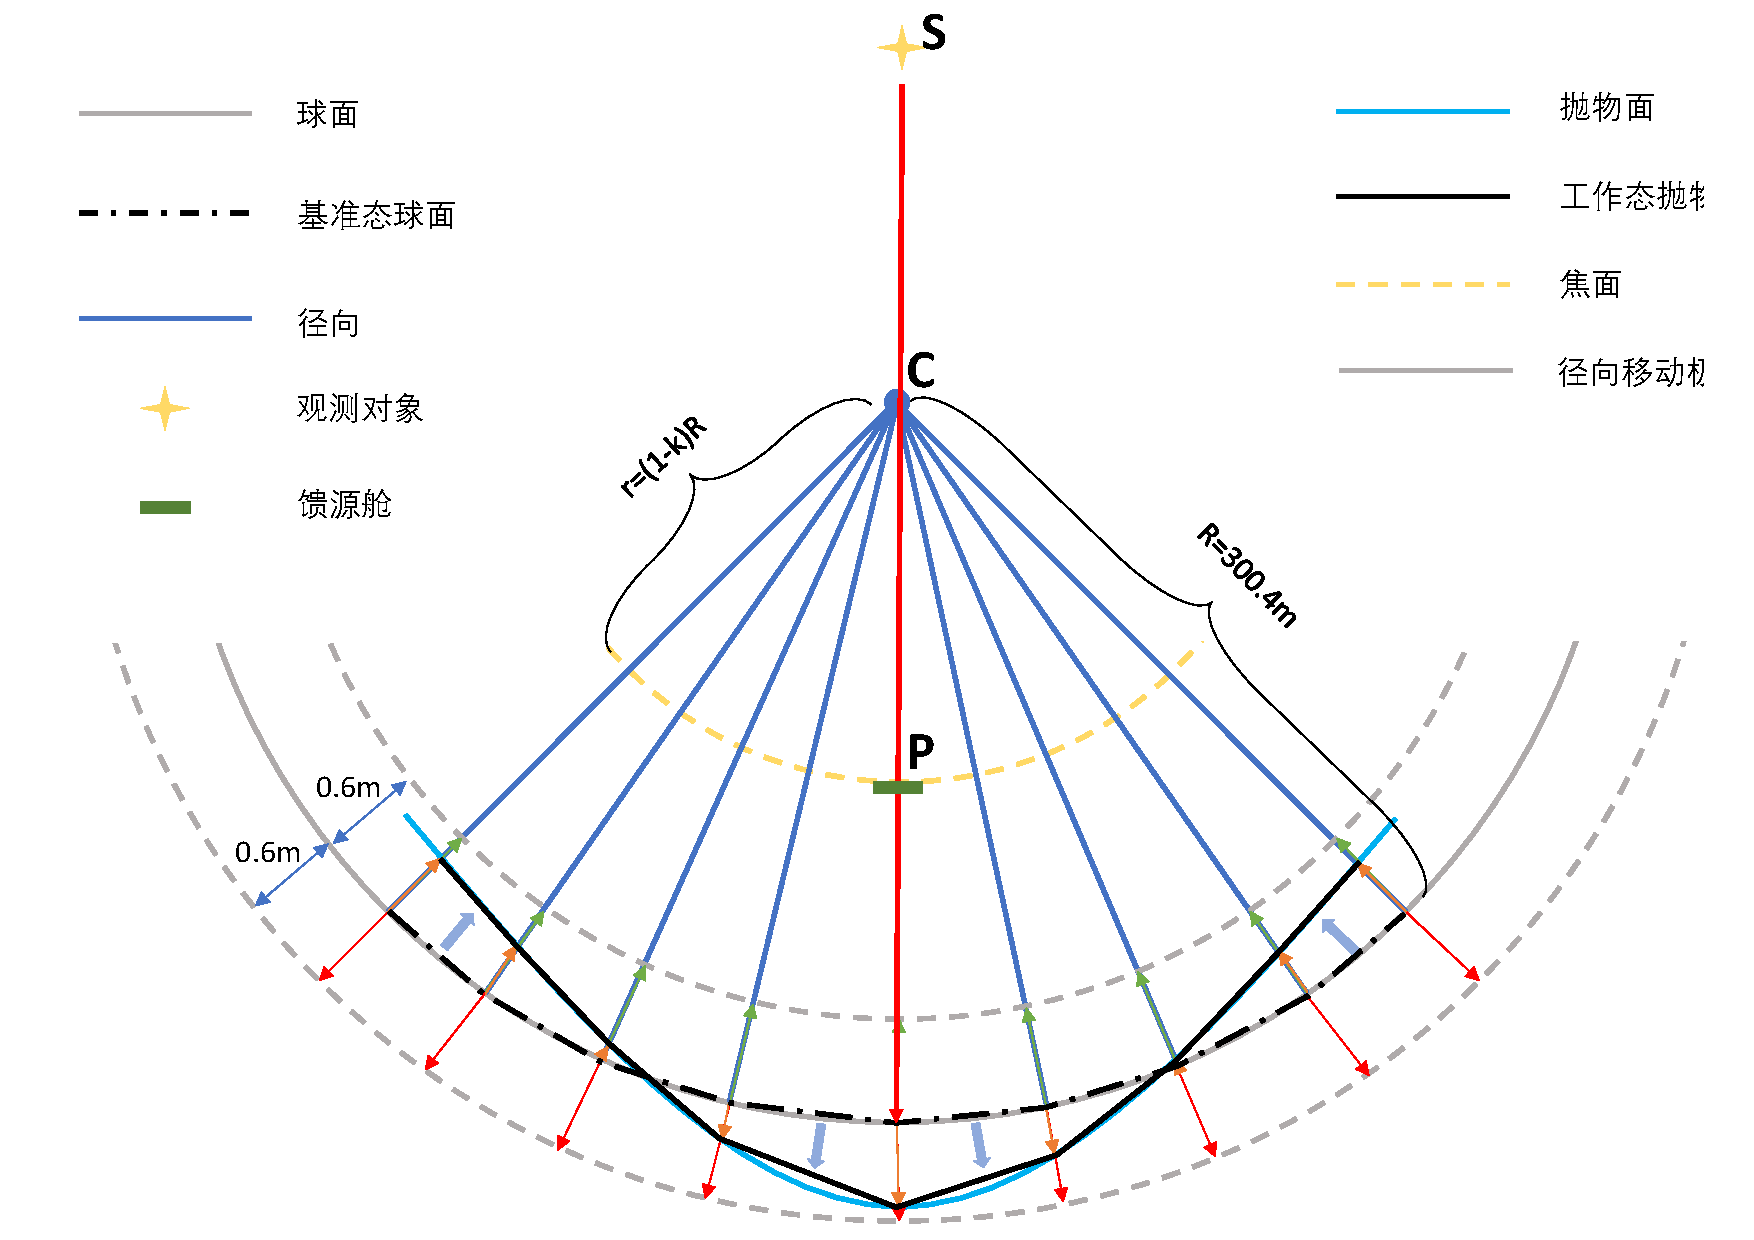
\includegraphics[width=1\textwidth]{模型示意图.pdf}
			\subcaption{移动区域示意图}
			\label{fig:sample-figure-a}
		\end{minipage}
		\begin{minipage}[c]{0.48\textwidth}
			\centering
			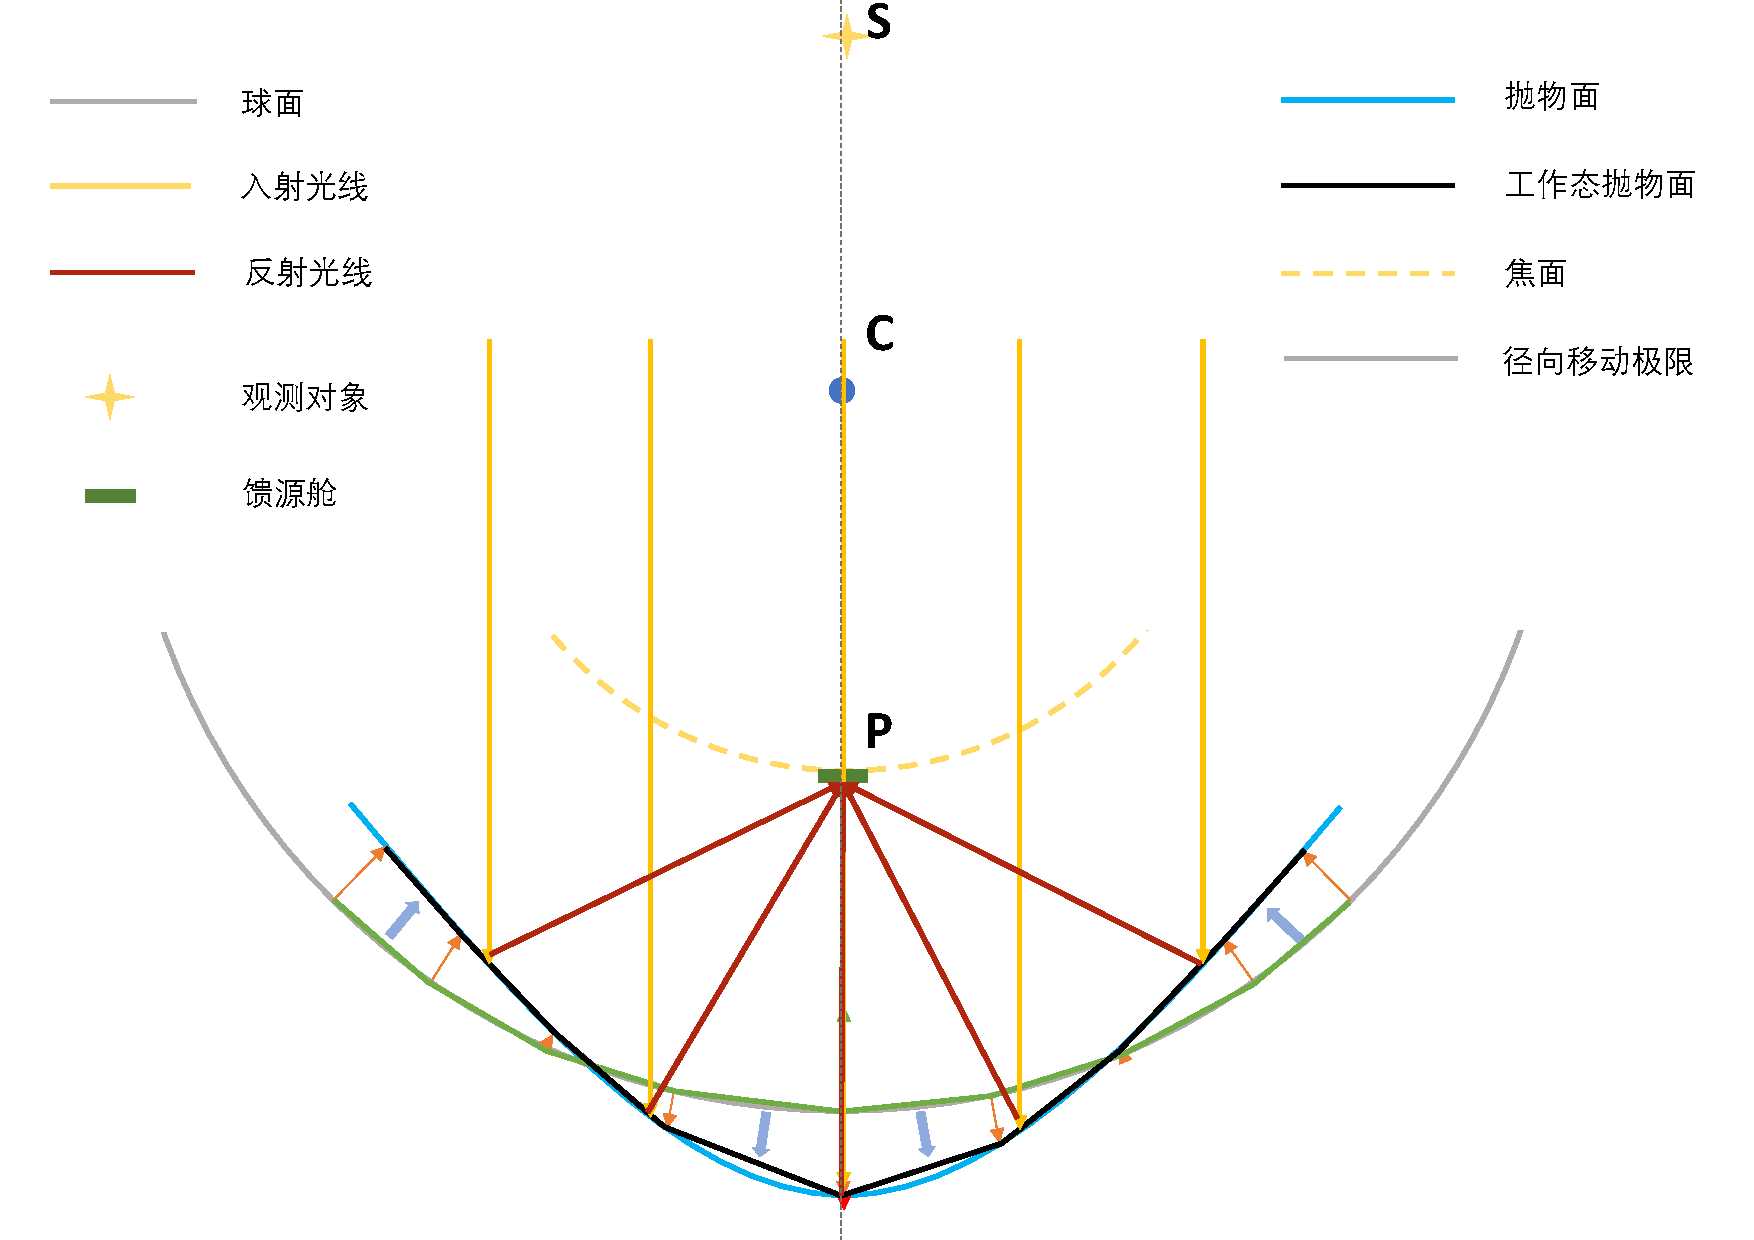
\includegraphics[width=1\textwidth]{反射示意图.pdf}
			\subcaption{光线反射示意图}
			\label{fig:sample-figure-b}
		\end{minipage}
		\caption{示意图}
		\label{fig:sample-figure}
	\end{figure}

	主索节点之间的主索长度变化不超过$0.07\%$。

	天体S的方位用方位角$\alpha$和仰角$\beta$来表示。

	问题1:待观测天体S位于基准球面正上方,即$\alpha=0°$,$\beta=90°$时,在满足主索长度变化限度和促动器伸缩范围的条件下,确定理想抛物面。

	问题2:待观测天体S位于$\alpha=36.795°$,$\beta=78.169°$时,在满足上述约束条件的前提下,确定理想抛物面;建立反射面板调节模型,刻画促动器的伸缩量,使实际情况下的工作台抛物面尽可能贴近该理想抛物面。

	问题3:基于问题2的反射面板调节模型,计算调节后馈源舱的接收比,即馈源舱有效区域接收到的反射信号与300米口径工作抛物面内的反射信号之比,并与基准态球面的接收比作比较。

	\section{问题分析}
	\subsection{问题1}
	天体S位于基准球面正上方,对应的工作态抛物面以$z$轴为对称轴,需要对以$z$轴为中心300m口径范围内的反射面板和与其相关的主索节点进行计算。写出以$z$轴为对称轴的抛物面方程,由于知道抛物面焦点位于焦面上这一条件,可知其仅由一个待定参数决定。为了确定这一参数,需要考虑反射面板对抛物面的拟合能力,这是因为主索长度变化限度和促动器伸缩范围这两条约束条件限制了反射面板不能完美地拟合理想抛物面。拟合是一个有较复杂约束的较大规模优化问题,由于索网分布为5个角度相等、呈中心对称的扇区,因此计算时可以利用对称性来减小计算量;另外也可以通过一些近似处理对问题进行简化。

	\subsection{问题2}
	问题在第一问的条件的基础上,将天体S的位置修改为$\alpha = 36.795^\circ$, $\beta = 78.169^\circ$。在求解问题1时所利用的对称性,在本题中无法继续利用。但对于不利用对称性的算法和模型,我们仅需是在第一问的基础上做一次坐标变换,则转化后的问题和第一问完全相同。在新坐标系下得到解后,只需做相反的坐标变换。在此基础上,问题还要求我们确定各个促动器的伸缩量以使反射面尽可能地贴近理想抛物面,我们便需要定义一个变量来刻画反射面接近理想抛物面的程度,并求解在前述约束条件下关于该变量的最优化模型。

	\subsection{问题3}
	问题要求计算基于问题2反射面板调节方案的调节后馈源舱接收比,并将其与基准态球面的接收比做对比,这要求我们建立信号传播的数学模型,模拟信号经反射面板反射后的传播,并计算反射到馈源舱有效接收区域(口径1m圆形区域)的比例,计算过程中需要用到计算几何的知识。


	\section{假设与符号}
	\subsection{模型假设}
	\begin{enumerate}
		\item 信号在工作抛物面300m口径范围内均匀分布;
		\item 信号经反射面板反射不发生损失;
		\item 忽略馈源舱对信号的阻挡;
		\item 主索节点不发生切向位移;
		\item 下拉索长度固定;
		\item 忽略重力、内力对反射面板和索网的影响;
		\item 温度变化、光照射等因素不会使索网产生形变;
	\end{enumerate}

	\subsection{符号说明}
	\begin{table}[!htbp]
		\caption{符号说明}\label{tab:001} \centering
		\begin{tabular}{ccc}
			\toprule[1.5pt]
			符号 & 含义 & 单位\\
			\midrule[1pt]
			$R$ & 基准态球面半径 & $m$ \\
			$B_{i}, G_{i}, A_{i}$ & 基准态、实际、理想节点 & $ $ \\
			$\lambda_i$ & 促动器伸长量 & $ $ \\
			$\vec{v_i}$ & 单位径向方向向量 & $$ \\
			$\theta$ & 相邻节点关于球心的夹角 & $rad$ \\
			$\Delta_i$ & 节点实际位置与理想位置的(径向)距离 & $m$ \\
			$\phi_\Delta, \phi_\cap$ & 投影平面上信号投影面积和接收面积 & $m^2$ \\
			$S_\Delta, S_\cap$ & 接收平面上信号投影面积和接收面积 & $m^2$ \\
			$\eta$ & 接收比 & $$ \\
			\bottomrule[1.5pt]
		\end{tabular}
	\end{table}


	\section{问题一模型建立与求解}
	\subsection{模型建立}
	\subsubsection{理想抛物面方程及约束条件}
	问题一所给出的天体S位于$\alpha=0°$,$\beta=90°$位置,因此理想抛物面应以z轴为对称轴,其方程为:
	\begin{equation}
		x^2 + y^2 + 2pz + c = 0
		\label{eq:paraboloid}
	\end{equation}
	其中$|p|$为焦准距。抛物面的焦点位于$(0, 0, -\frac{p}{2}-\frac{c}{2p})$。
	
	
	馈源舱位于天体S与球面中心C的连线SC与焦面的交点P处,其中心坐标为$(0, 0, F-R)$。
	为使电磁波信号经抛物面反射后尽可能多地被馈源舱有效接收区域接收,应使抛物面的焦点与馈源舱中心重合,因此有:
	\begin{equation}
		-\frac{p}{2}-\frac{c}{2p} = F-R
		\label{eq:foci}
	\end{equation}
	其中$R = 300.4m$,这一数值是通过分析节点坐标数据和查阅有关文献得到的,$F = 0.466R$。这说明理想抛物面可由参数 $p$ 唯一确定。
	
	根据题给要求及相关参数可知,促动器在径向上的伸缩范围为$-0.6 \textasciitilde +0.6$m。假设在促动器及与之相连的下拉索的控制下,对应下拉索相连的主索节点不发生切向位移,记节点与球心连线$B_{i} C$的单位方向向量为$\vec{v}_i$,节点的位移可表示为$\lambda_i \vec{v}_i$。位移大小为$\lambda_i|\vec{v}_i| = \lambda_i$,故得到第一个约束条件:
	\begin{equation}
		-0.6 \leq \lambda_i \leq 0.6
		\label{eq:bound2}
	\end{equation}

	对基准态任意节点$B_{i}(x_i, y_i, z_i)$,与其在基准态球面相邻的节点$B_{j}$之间的距离为$d_{ij} = \sqrt{(x_i-x_j)^2+(y_i-y_j)^2+(z_i-z_j)^2}$。这一距离可视为节点$B_{i}B_{j}$之间主索的长度,由于主索长度的变化幅度不超过0.07\%,我们得到了第二个约束条件:
	\begin{equation}
		\frac{\Delta d_{ij}}{d_{ij}}< 0.0007
		\label{eq:bound1}
	\end{equation}
	
	相邻两点$B_{i},B_{j}$调整前后如图\ref {fig:before_after}所示。即两直线夹角为$\theta$,由余弦定理,调整后的主索$G_{i}G_{j}$的长度为$\sqrt{(R-\lambda_i)^2+(R-\lambda_j)^2-2(R-\lambda_i)(R-\lambda_j)\cos\theta}$。调整前的主索$B_{i}B_{j}$的长度为$\sqrt{2R^2(1-\cos\theta)}$。故式\ref {eq:bound1}可改写为:
	$$0.9993 \leq \frac{\sqrt{(R-\lambda_i)^2+(R-\lambda_j)^2-2(R-\lambda_i)(R-\lambda_j)\cos\theta}}{\sqrt{2R^2(1-\cos\theta)}} \leq 1.0007$$
	平方并化简得:
	\begin{equation}
		0.9993^2 \leq 1+\frac{\lambda_i^2+\lambda_j^2}{2R^2(1-\cos\theta)}-\frac{\lambda_i+\lambda_j}{R} \leq 1.0007^2
		\label{eq:bound1_transform}
	\end{equation}
	
	\begin{figure}[!h]
		\centering
		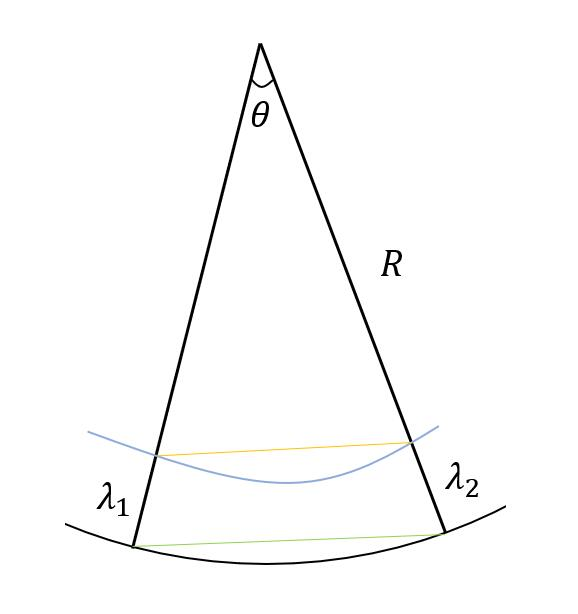
\includegraphics[height=0.4\textwidth]{before_after.jpg} % 表示缩放到文本行的 0.4 倍宽
		\caption{节点调整前后}
		\label{fig:before_after}
	\end{figure}
	
	
	接下来考虑应该调整哪些节点。题目给出的馈源舱照明区域为$300m$口径圆形区域,在该范围内的节点在工作态下应尽可能按照理想抛物面排列,故至少在$300m$口径范围内的节点应被调整位置;若调整$300m$口径范围之外的节点至抛物面位置,考虑到抛物面的斜率随着点远离对称轴的距离增大而增大,越远离对称轴的点从球面上调整至抛物面所需移动的距离越长,不利于满足约束条件\ref {eq:bound1}和\ref {eq:bound2}。基于这种考虑,我们在处理工作抛物面的形成时仅调整$300m$口径照明范围之内的节点。

	\subsubsection{双层优化模型}
	
	\textbf{内层优化}
	
	给定参数 $p$,我们可以确定一个理想抛物面。在不考虑伸缩限制的情况下,主索节点可以沿着它的伸缩方向到达理想抛物面,称到达的位置为理想点,记为 $A_i$,称对应的伸缩量为理想伸缩量,记为 $\mu_i$。如图\ref{fig:g_ideal}所示。
	
	\begin{figure}[!h]
		\centering
		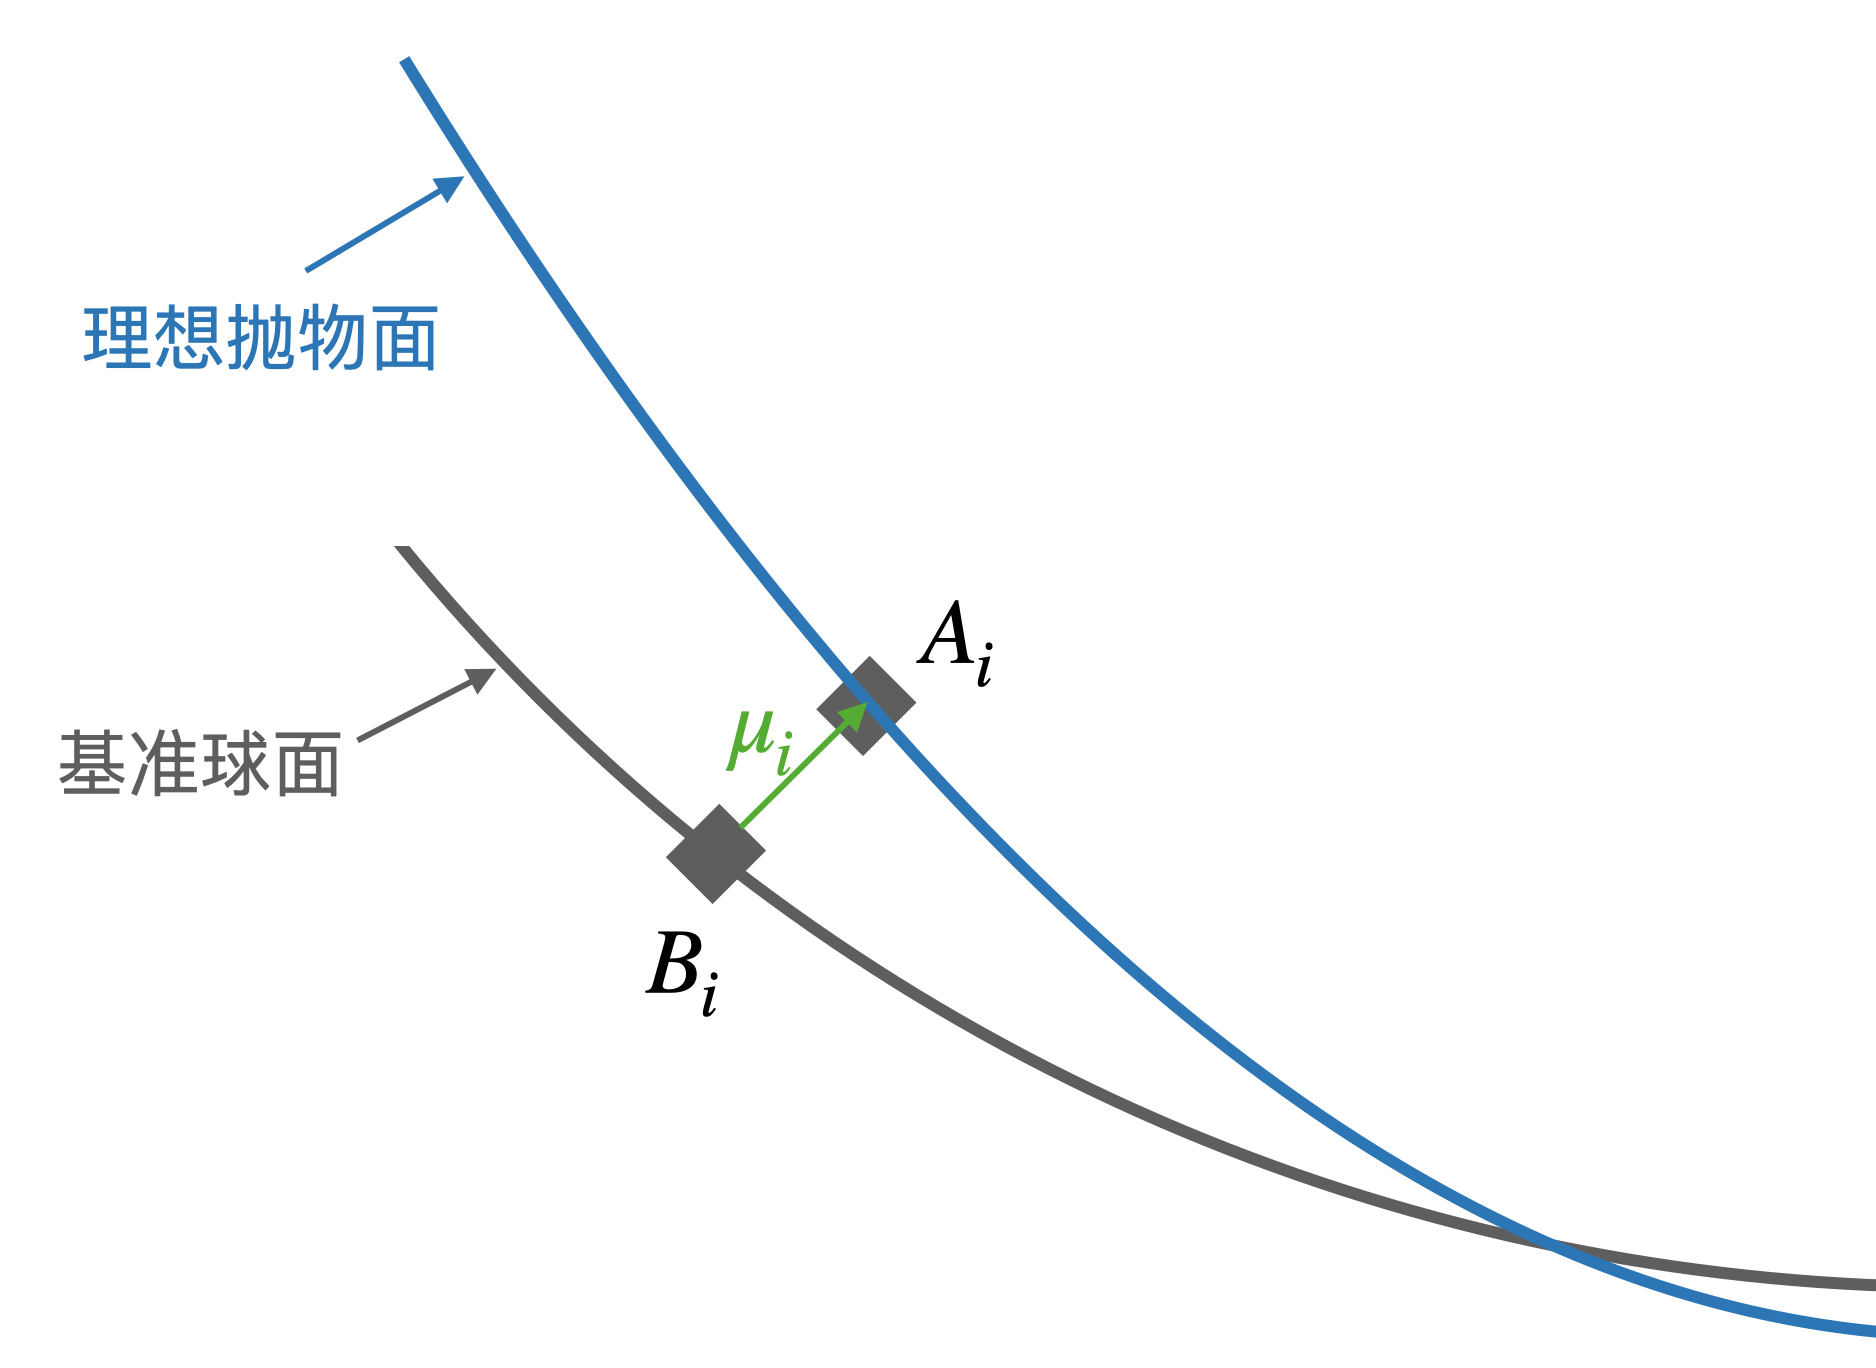
\includegraphics[height=0.4\textwidth]{伸缩示意图.png} % 表示缩放到文本行的 0.4 倍宽
		\caption{节点在理想抛物面上的位置}
		\label{fig:g_ideal}
	\end{figure}

	实际形成抛物面时,难以保证主索节点均在理想抛物面上。记实际形成工作抛物面后节点的位置为$G_{i}$,$|{G_{i}A_{i}}| = |\lambda_i-\mu_i|$为实际位置和理想位置的(径向)距离。以所有节点实际位置和理想位置的距离平方和作为工作抛物面对理想抛物面贴近程度的度量函数,可以建立如下的最优化模型:

	\begin{align}
		&\min_{\lambda_i} \sum_{i\in\text{Area}}(\lambda_i-\mu_i)^2, \notag \\
		&\text{s.t.}\begin{cases}
			-0.6 \leqslant \lambda_i \leqslant 0.6, & i=1,2,\cdots, n\\
			0.9993^2 \leqslant 1+\dfrac{\lambda_i^2+\lambda_j^2}{2R^2(1-\cos\theta)}-\dfrac{\lambda_i+\lambda_j}{R} \leqslant 1.0007^2,&(i,j)\in\text{AdjPairs}\\
		\end{cases}
		\label {opt:optimization_1}
	\end{align}

	其中,$\text{Area}$ 表示口径$300m$内的节点集合,$\text{AdjPairs}$ 表示相邻节点对的集合。

	\textbf{外层优化}
	
	对于一个特定的抛物面参数$p$,内层优化问题的最终结果指示了反射面板与理想抛物面的最大拟合程度 $\text{Fit}(p)$。当我们改变 $p$ 时,抛物面发生改变,反射面板的最大拟合程度也随之改变。我们认为,最优的理想抛物面应使得反射面板的拟合程度最大,因此以最小化 $\text{Fit}(p)$ 为目标,我们可以得到最优理想抛物面参数 $p^*$:
	
	\begin{equation}
		p^*=\arg\min_p \text{Fit}(p)
	\end{equation}

	\subsection{模型求解}
	\subsubsection {数据预处理}
		根据题目给出的条件和数据,我们围绕节点无切向位移这一假设分析了下拉索与径向的夹角,发现除表\ref{tab:abnormal}所列出节点外,其余节点夹角均在$0.05^\circ$内。作出夹角异常点分布图\ref {fig:abnormal},可见其分布无明显规律。进一步分析数据可知,所有促动器伸缩方向与径向向量保持高度一致,因而我们以促动器伸缩方向作为异常节点的方向向量,这样可以保证所有待处理的节点严格按照题给条件和本文所作假设在径向上移动而不产生切向位移。
		\begin{table}[!h]
		    \centering
		    \begin{tabular}{|l|l|l|l|l|l|}
		    \hline
		        异常点编号 & D155 & E140 & A132 & B286  & B285 \\ \hline
		        异常夹角(度) & 36.92258762 & 30.75418587 & 25.15579224 & 15.71386879 & 13.73493399 \\ \hline
		        异常点编号 &  D69  & B284  & B287  & A385  & B288 \\ \hline
		        异常夹角(度) & 13.67256016 & 10.06280305 & 9.41951411 & 8.60924787 & 8.07094271 \\ \hline
		    \end{tabular}
	    	\caption{异常点数据}
	    	\label{tab:abnormal}
		\end{table}
		
		\begin{figure}[!h]
			\centering
			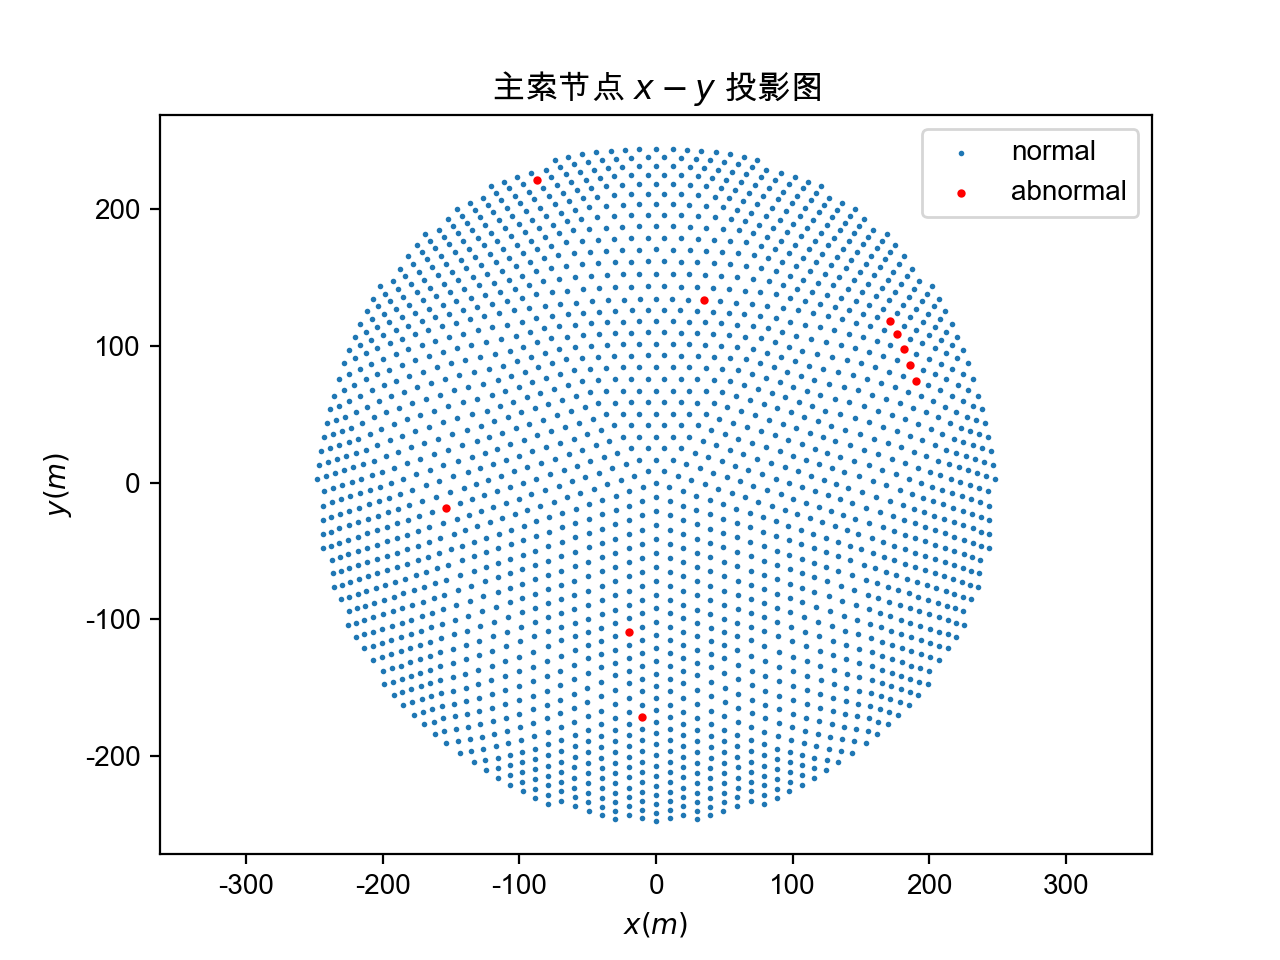
\includegraphics[height=0.4\textwidth]{abnormal.png} % 表示缩放到文本行的 0.4 倍宽
			\caption{异常节点数据及分布}
			\label{fig:abnormal}
		\end{figure}

	\subsubsection {内层优化问题求解}
	
		由\ref {opt:optimization_1}式确定的内层优化模型是一个复杂约束的高维非线性规划问题,其维数经计算可多达706维,一般的优化方法难以直接求解。解决思路有二,一是利用球面的对称性,将节点进行分组计算,各组内的节点共用决策变量,从而降低维度;二是将复杂约束的非线性规划问题通过近似处理简化为一个二次规划问题,可以在不损失维度的情况下计算出优化解。
		
		\textbf{分组优化}
		
		观察分析各主索节点的编号规律,得知节点可以分为关于z轴中心对称的5个扇区,且具有层次结构,如图 \ref {fig:sector_layer}所示。
		
		\begin{figure}[!h]
			\centering
			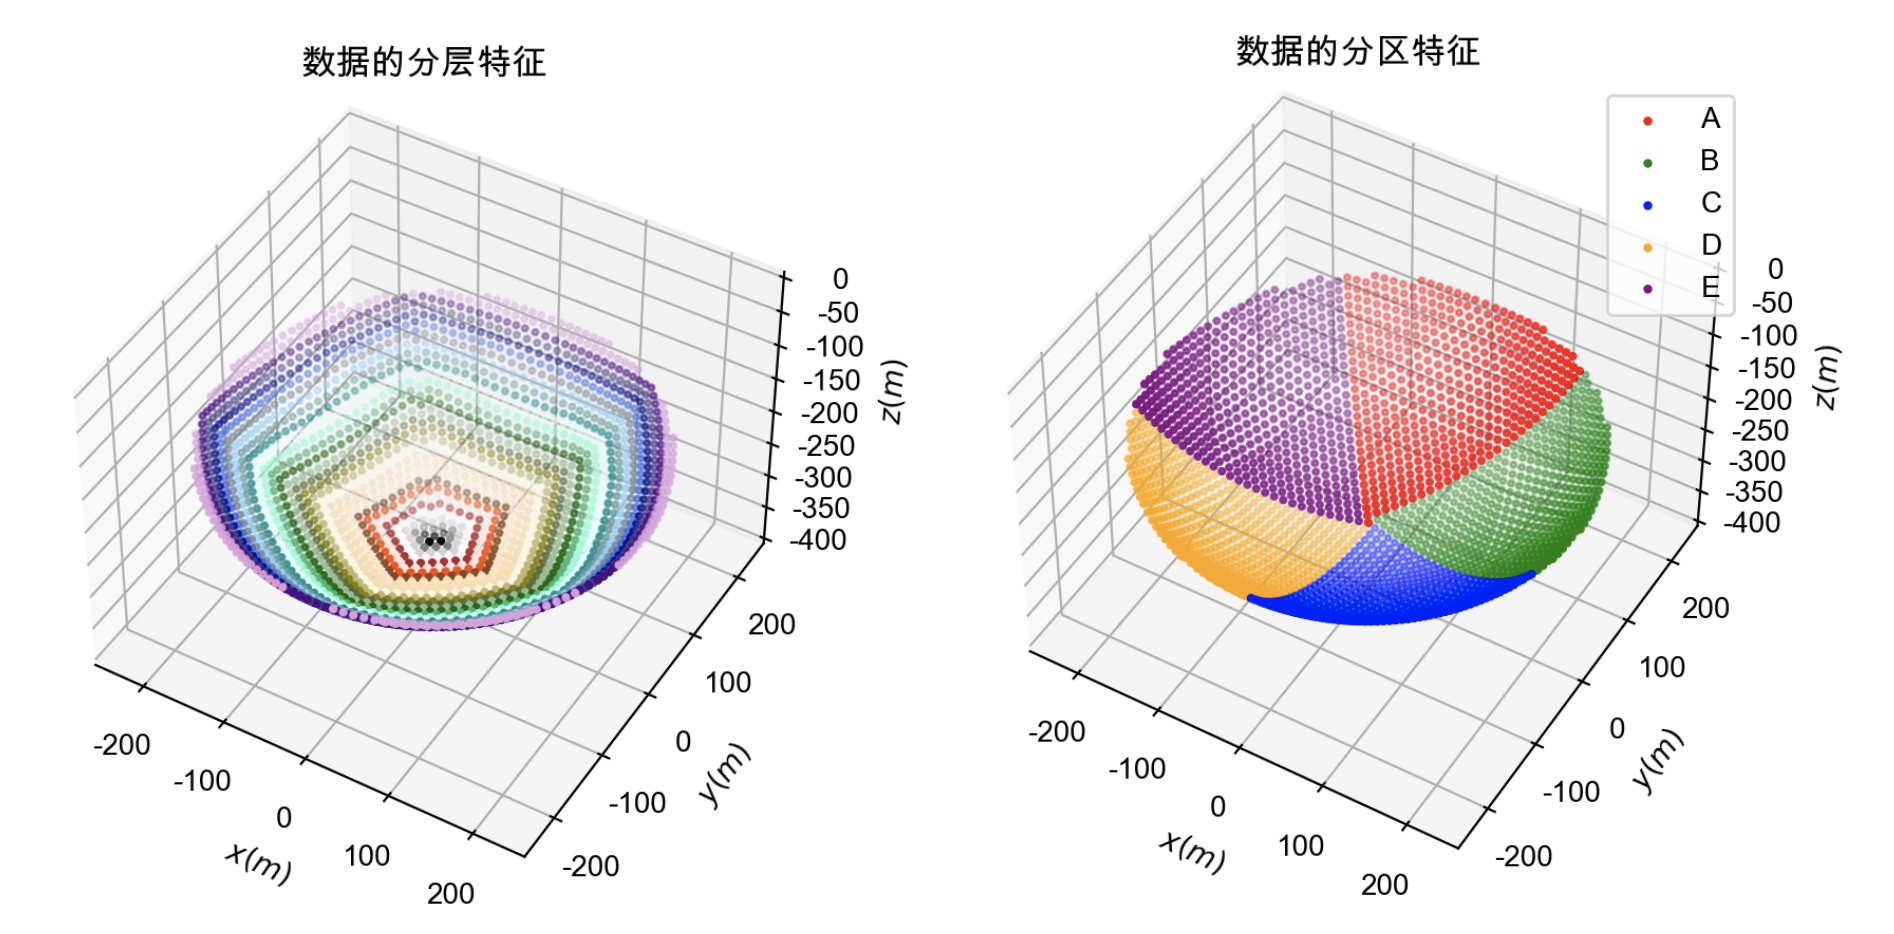
\includegraphics[height=0.4\textwidth]{sector_layer.png} % 表示缩放到文本行的 0.4 倍宽
			\caption{节点分层与分区特征}
			\label{fig:sector_layer}
		\end{figure}

		基于对称性,我们将同一层的节点分为一组,这使得维度大大减小至 $17$,因而使用常用的非线性优化算法也能快速求出\ref{opt:optimization_1}的解。
		
		\textbf{近似简化为二次规划}
		
		分析数据可知相邻节点之间的角度平均为 $2.17^\circ$,最大 $3.19^\circ$,这是一个较小的角度,且促动器伸缩范围 $\pm 0.6m$ 与半径 $300.4m$ 有 $3$ 个数量级的差异,因此,相邻节点伸缩方向可近似为平行方向。在此近似下,相邻节点距离总是增大,且
		$$
		{d'_{ij}}^2=(\lambda_i-\lambda_j)^2+d_{ij}^2\notag
		$$
		于是式 $\ref{eq:bound1}$ 转化为:
		$$
		\left|\frac{d'_{ij}-d_{ij}}{d_{ij}}\right|=\sqrt{1+\frac{(\lambda_i-\lambda_j)^2}{d_{ij}^2}}-1\leqslant 0.07\%\notag
		$$
		由于 $(\lambda_i-\lambda_j)^2$ 与 $d_{ij}^2$ 相差两个数量级,利用泰勒展开式 $(1+x)^\alpha=1+\alpha x+\frac{\alpha(\alpha-1)}{2}x^2+\cdots$ 并取一阶近似,得到转换后的约束条件:
		$$
		\frac{(\lambda_i-\lambda_j)^2}{2d^2_{ij}}\leqslant 0.07\%\notag
		$$
		如上文所述,此简化近似中节点距离总是增大,无法对距离减小的情况做约束。因此,引入一个伸缩上界变量 $\Lambda_i$ 代替 $0.6$,表示第 $i$ 个主索节点的伸缩范围,则当 $\Lambda_i$ 足够小时,一定有满足约束条件的解。于是问题最终转化为:
		
		\begin{align}
			&\min_{\lambda_i} \sum_{i\in\text{Area}}(\lambda_i-\mu_i)^2\notag\\
			&\text{s.t.}\begin{cases}
					|\lambda_i|\leqslant\Lambda_i&i=1,2,\ldots\\
					|\lambda_i-\lambda_j|\leqslant \sqrt{0.0014}d_{ij}&(i,j)\in\text{AdjPairs}
					\end{cases}
		\end{align}
		
		这是一个凸二次规划问题且具有唯一最小值,因而即便规模较大,也能很快地求出最优解。

		在实际求解中,$\Lambda_i$ 初始取值 $0.6$,当解不满足约束条件时,将不满足条件的主索节点的 $\Lambda$ 乘上一比例因子,使得 $\Lambda$ 依指数下降,然后重新求解直至满足约束条件。
		
	\subsubsection{外层优化问题求解}
		
		针对 A0 号主索节点,由于 0.6m 伸缩量的限制,其 $z$ 坐标范围控制在 $-300.4\pm0.6$ 的范围中,由于它将拟合抛物线顶点,因而可以接触参数 $p$ 的大致范围 $[-285, -275]$.
		
		对 $p$ 采用变步长枚举法,在该范围内逐步缩小搜索范围与步长,迭代图像如\ref{fig:p_step}所示。
		
		\begin{figure}[!h]
			\centering
			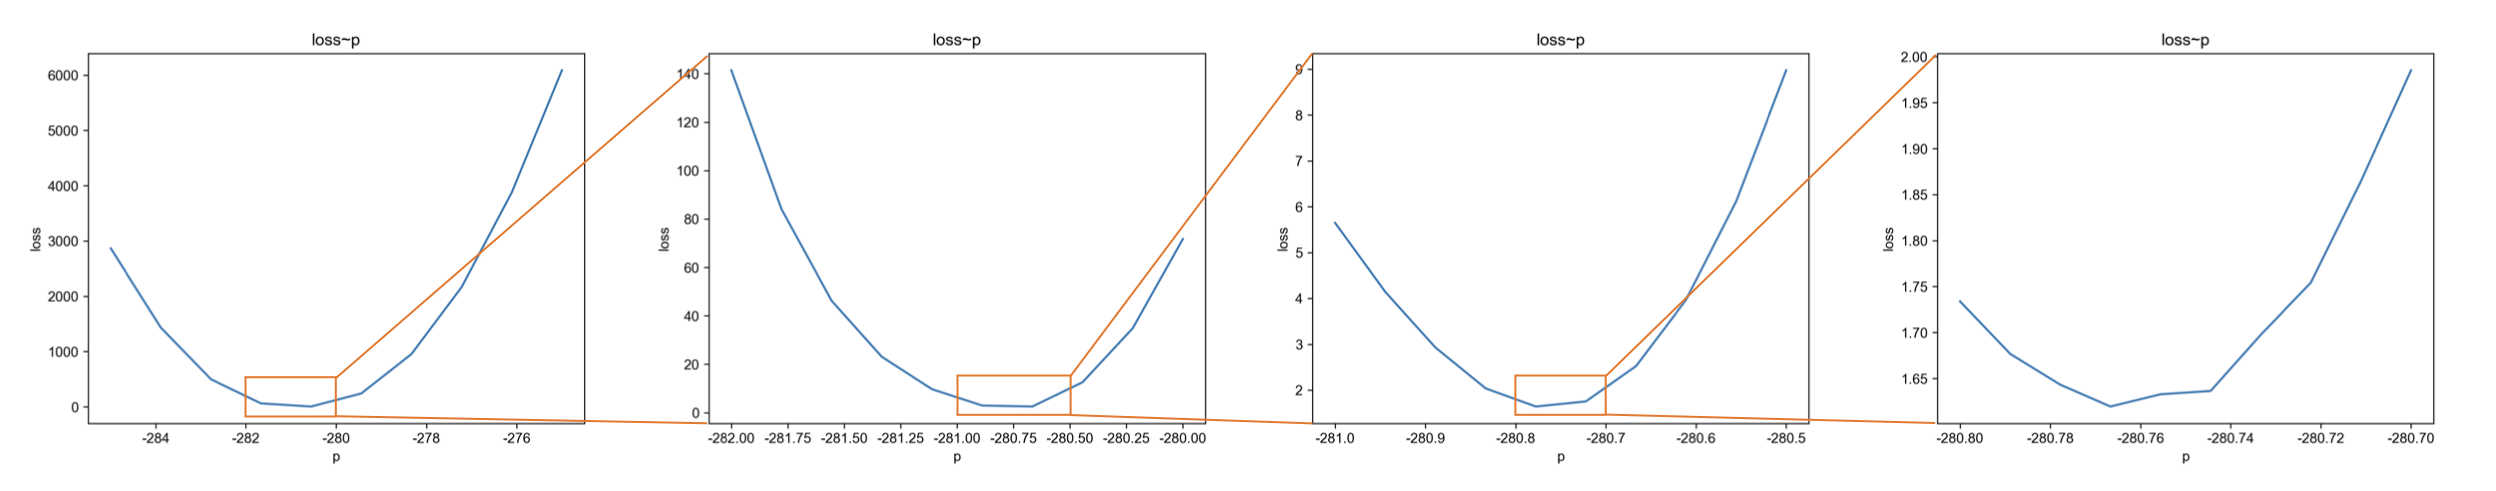
\includegraphics[width=\textwidth]{p_step.png} % 表示缩放到文本行的 0.4 倍宽
			\caption{对 $p$ 变步长枚举}
			\label{fig:p_step}
		\end{figure}
	
		观察枚举结果可知,$\text{Fit}(p)$ 基本是一个凸函数,可以使用一般的凸优化方法求解。
		
		针对两种不同的内层优化方法,它们分别对应的拟合结果如图\ref{fig:curveT1}所示,抛物线参数与 $\text{Fit}(p)$ 拟合程度如表\ref{tab:resultT1}所示。
		
		\begin{figure}[!h]
			\centering
			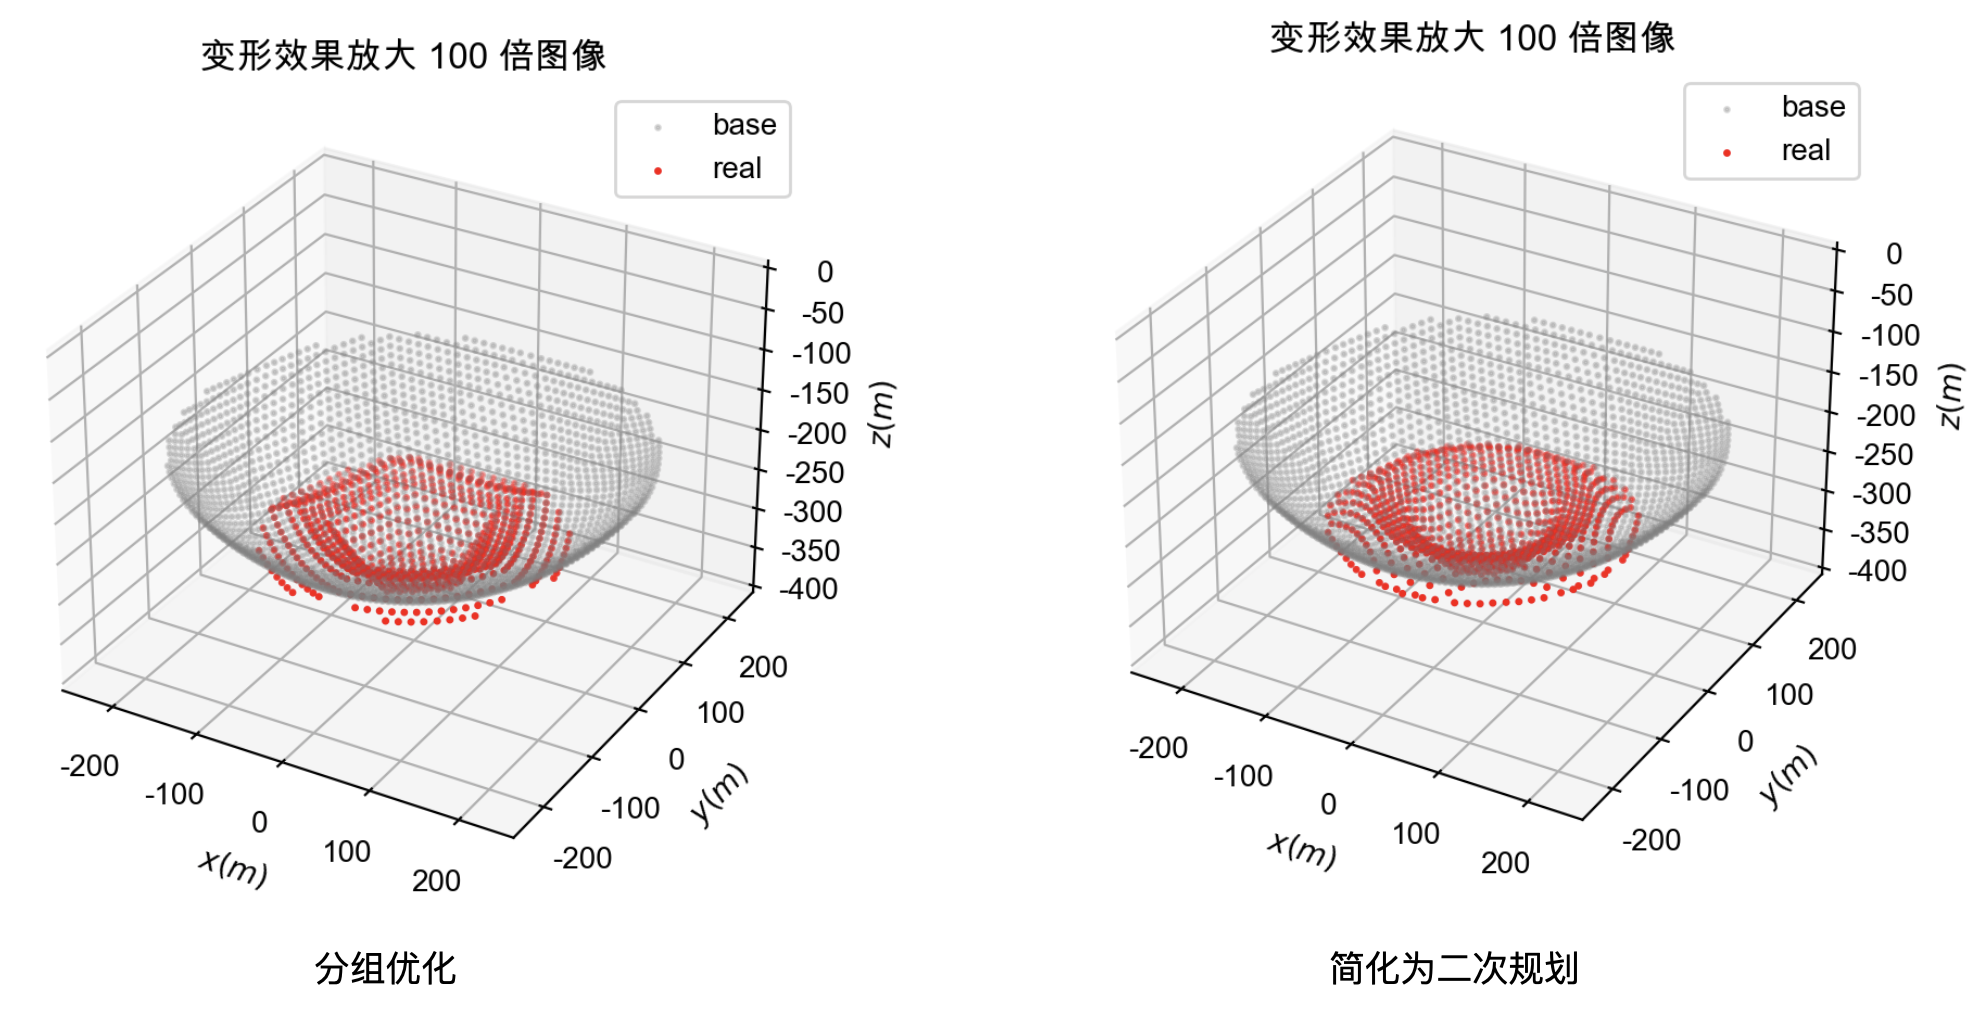
\includegraphics[height=0.4\textwidth]{curveT1.png} % 表示缩放到文本行的 0.4 倍宽
			\caption{两种内层方法的拟合结果}
			\label{fig:curveT1}
		\end{figure}
	
		\begin{table}[!h]
			\centering
			\begin{tabular}{|l|l|l|l|}
				\hline
				方法 & p & c & Fit(p) \\ \hline
				分组优化 & -280.78486814 & -168923.5652241226 & 5.214526581640151 \\ \hline
				二次规划 & -280.76746957 & -168908.21308196918 & 1.6156233191701248 \\ \hline
			\end{tabular}
			\caption{问题一结果}
			\label{tab:resultT1}
		\end{table}
	
		从结果可见,无论是从 $\text{Fit}(p)$ 的数值角度还是图像的直观角度,分组优化的效果都显著差于简化为二次规划的效果。又由于我们采用的分组方法——按层分组——只在如问题一的对称情形下适用,因此我们继续采用二次规划方法解决后续问题。
		

	\section {问题二模型建立与求解}
	\subsection{模型建立}
	\subsubsection {基于坐标变换的双层优化模型推广}
		%直线SC的单位方向向量为$(\cos\beta_0\cos\alpha_0, \cos\beta_0\sin\alpha_0, \sin\beta_0)$,则SC直线方程的参数形式可写成
		%\begin{align}
		%	&\begin{cases}
		%			x = t\cos\beta_0\cos\alpha_0\\
		%			y = t\cos\beta_0\sin\alpha_0\\
		%			z = t\sin\beta_0
		%		\end{cases}
		%\end{align}
		%其中$t$为参数。记准面与SC的交点对应的参数为$t_0$,给定p,可写出抛物面
		
		
		在问题一中所使用的双层优化模型仅适用于求解$\alpha =0, \beta = 90°$的特殊情形。考虑$\alpha = \alpha_0, \beta = \beta_0$的一般情形,以直线SC为对称轴,理想抛物面和基准球面仍然关于它中心对称,因而在问题一中求解模型的方法,经过坐标旋转变换后可以适用于问题二。设空间内一向量在原本坐标系中坐标为$(x,y,z)$,在以SC为z轴的新坐标系中坐标为$(x', y', z')$,根据坐标变换有:
		\begin{equation}
			\begin{pmatrix}
			    x' \\
			    y' \\
			    z' \\
			\end{pmatrix}=
			A^{-1}
			\begin{pmatrix}
			    x \\
			    y \\
			    z \\
			\end{pmatrix}
			\label{eq:coordinate_transform}
		\end{equation}
		其中,$$A = \begin{pmatrix}
						    \sin\alpha & \cos\alpha\sin\beta & \cos\alpha\cos\beta \\
						    -\cos\alpha & \sin\alpha\sin\beta & \sin\alpha\cos\beta \\
						    0 & -\cos\beta & \sin\beta \\
						\end{pmatrix}$$
		
		描述径向伸缩量的标量$\lambda_i$不受坐标变换影响,相邻两点 $i,j$ 之间的距离 $d_{ij}$ 也不受坐标变换影响,因而我们的优化目标依旧是 \ref{opt:optimization_1} 不变。
		
	
	通过和问题一中相同的方法求解得到$\lambda_i$,进而可以求出新坐标系下主索节点变形后的坐标$G_i' = (x', y', z')^T$, 左乘坐标变换矩阵 $A$ 即可得到该点在原坐标系下的坐标$G_i = (x, y, z)^T$。
	
	\subsection {模型求解}
	\subsubsection {计算过程}
		设所有节点的初始位置信息为 $Q_{3\times n}$,其中 $n$ 表示点的数目,列向量 $\begin{pmatrix}x_i\\y_i\\z_i\end{pmatrix}$ 表示第 $i$ 个点的坐标,则所有节点坐标变换之后在新坐标系下的位置为
		\begin{align*}
		Q' &= A\cdot Q \\
		   &= \begin{pmatrix}
						    \sin\alpha & \cos\alpha\sin\beta & \cos\alpha\cos\beta \\
						    -\cos\alpha & \sin\alpha\sin\beta & \sin\alpha\cos\beta \\
						    0 & -\cos\beta & \sin\beta \\
						\end{pmatrix} \cdot
			\begin{pmatrix}
			x_1 & x_2 & \cdots & x_n\\
			y_1 & y_2 & \cdots & y_n\\
			z_1 & z_2 & \cdots & z_n
			\end {pmatrix}\\
			&= \begin{pmatrix}
			x_1' & x_2' & \cdots & x_n'\\
			y_1' & y_2' & \cdots & y_n'\\
			z_1' & z_2' & \cdots & z_n'
			\end {pmatrix}
		\end{align*}
		于此同时,原坐标系中入射角度为 $(\alpha, \beta)$ 的信号在新坐标系中可以看做沿 $z$ 轴负方向的射入的信号,因此可以直接使用问题 1的模型进行求解。由于变换后的坐标不再具有分区特征,因此只能使用二次规划模型进行求解。
		
		求解之后,对新坐标系下的所有节点施加逆变换,即可得到其在原坐标系下的坐标 $Q^*_{3\times n}$
		$$
		Q^* = A^{-1}\cdot Q'
		$$
	
	\subsubsection {求解流程图}
		\begin{figure}[!h]
			\centering
			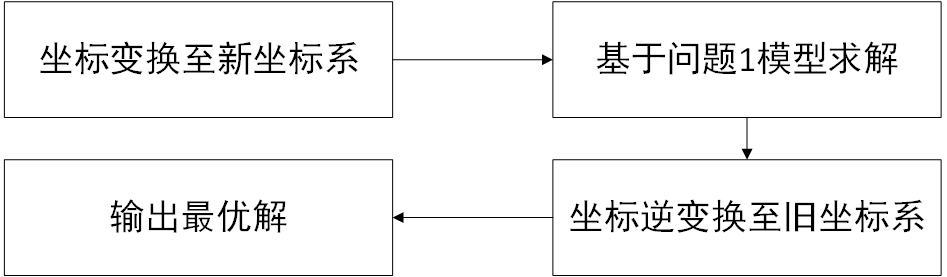
\includegraphics[width=0.6\textwidth]{Q2_process.png} % 表示缩放到文本行的 0.4 倍宽
			\caption{问题2求解流程}
		\end{figure}
	
	\subsubsection {求解结果}
		求解之后各点主索网编号、坐标以及对应促动器顶端伸缩量如下表,详细信息见附录文件
	
		\begin{table}[!htbp]
			\centering
			\begin{tabular}{ccc}
				\toprule[1.5pt]
				主索网节点标号 & 主索网节点位置坐标 & 促动器顶端伸缩量\\
				\midrule[1pt]
				A0 & (4.80e-14, 1.10e-14, -300.4176) & -0.017595514\\
				B1 & (6.1062511, 8.40487074, -300.14415) & 0.076099268\\
				\vdots & \vdots & \vdots\\
				D269 & (-148.91638, -131.96017, -225.33377) & -0.207675003\\
				\bottomrule[1.5pt]
			\end{tabular}
			\caption{调整信息表}
		\end{table}
	
		同时对数据结果进行了可视化处理
		
		\begin{figure}[!h]
			\centering
			\begin{minipage}[c]{0.48\textwidth}
				\centering
				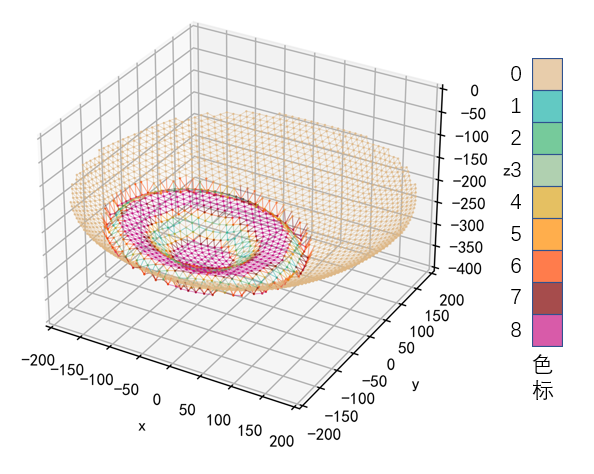
\includegraphics[width=1\textwidth]{rotate_diff.png}
				\subcaption{形变图}
				\label{rotate_diff}
			\end{minipage}
			\begin{minipage}[c]{0.48\textwidth}
				\centering
				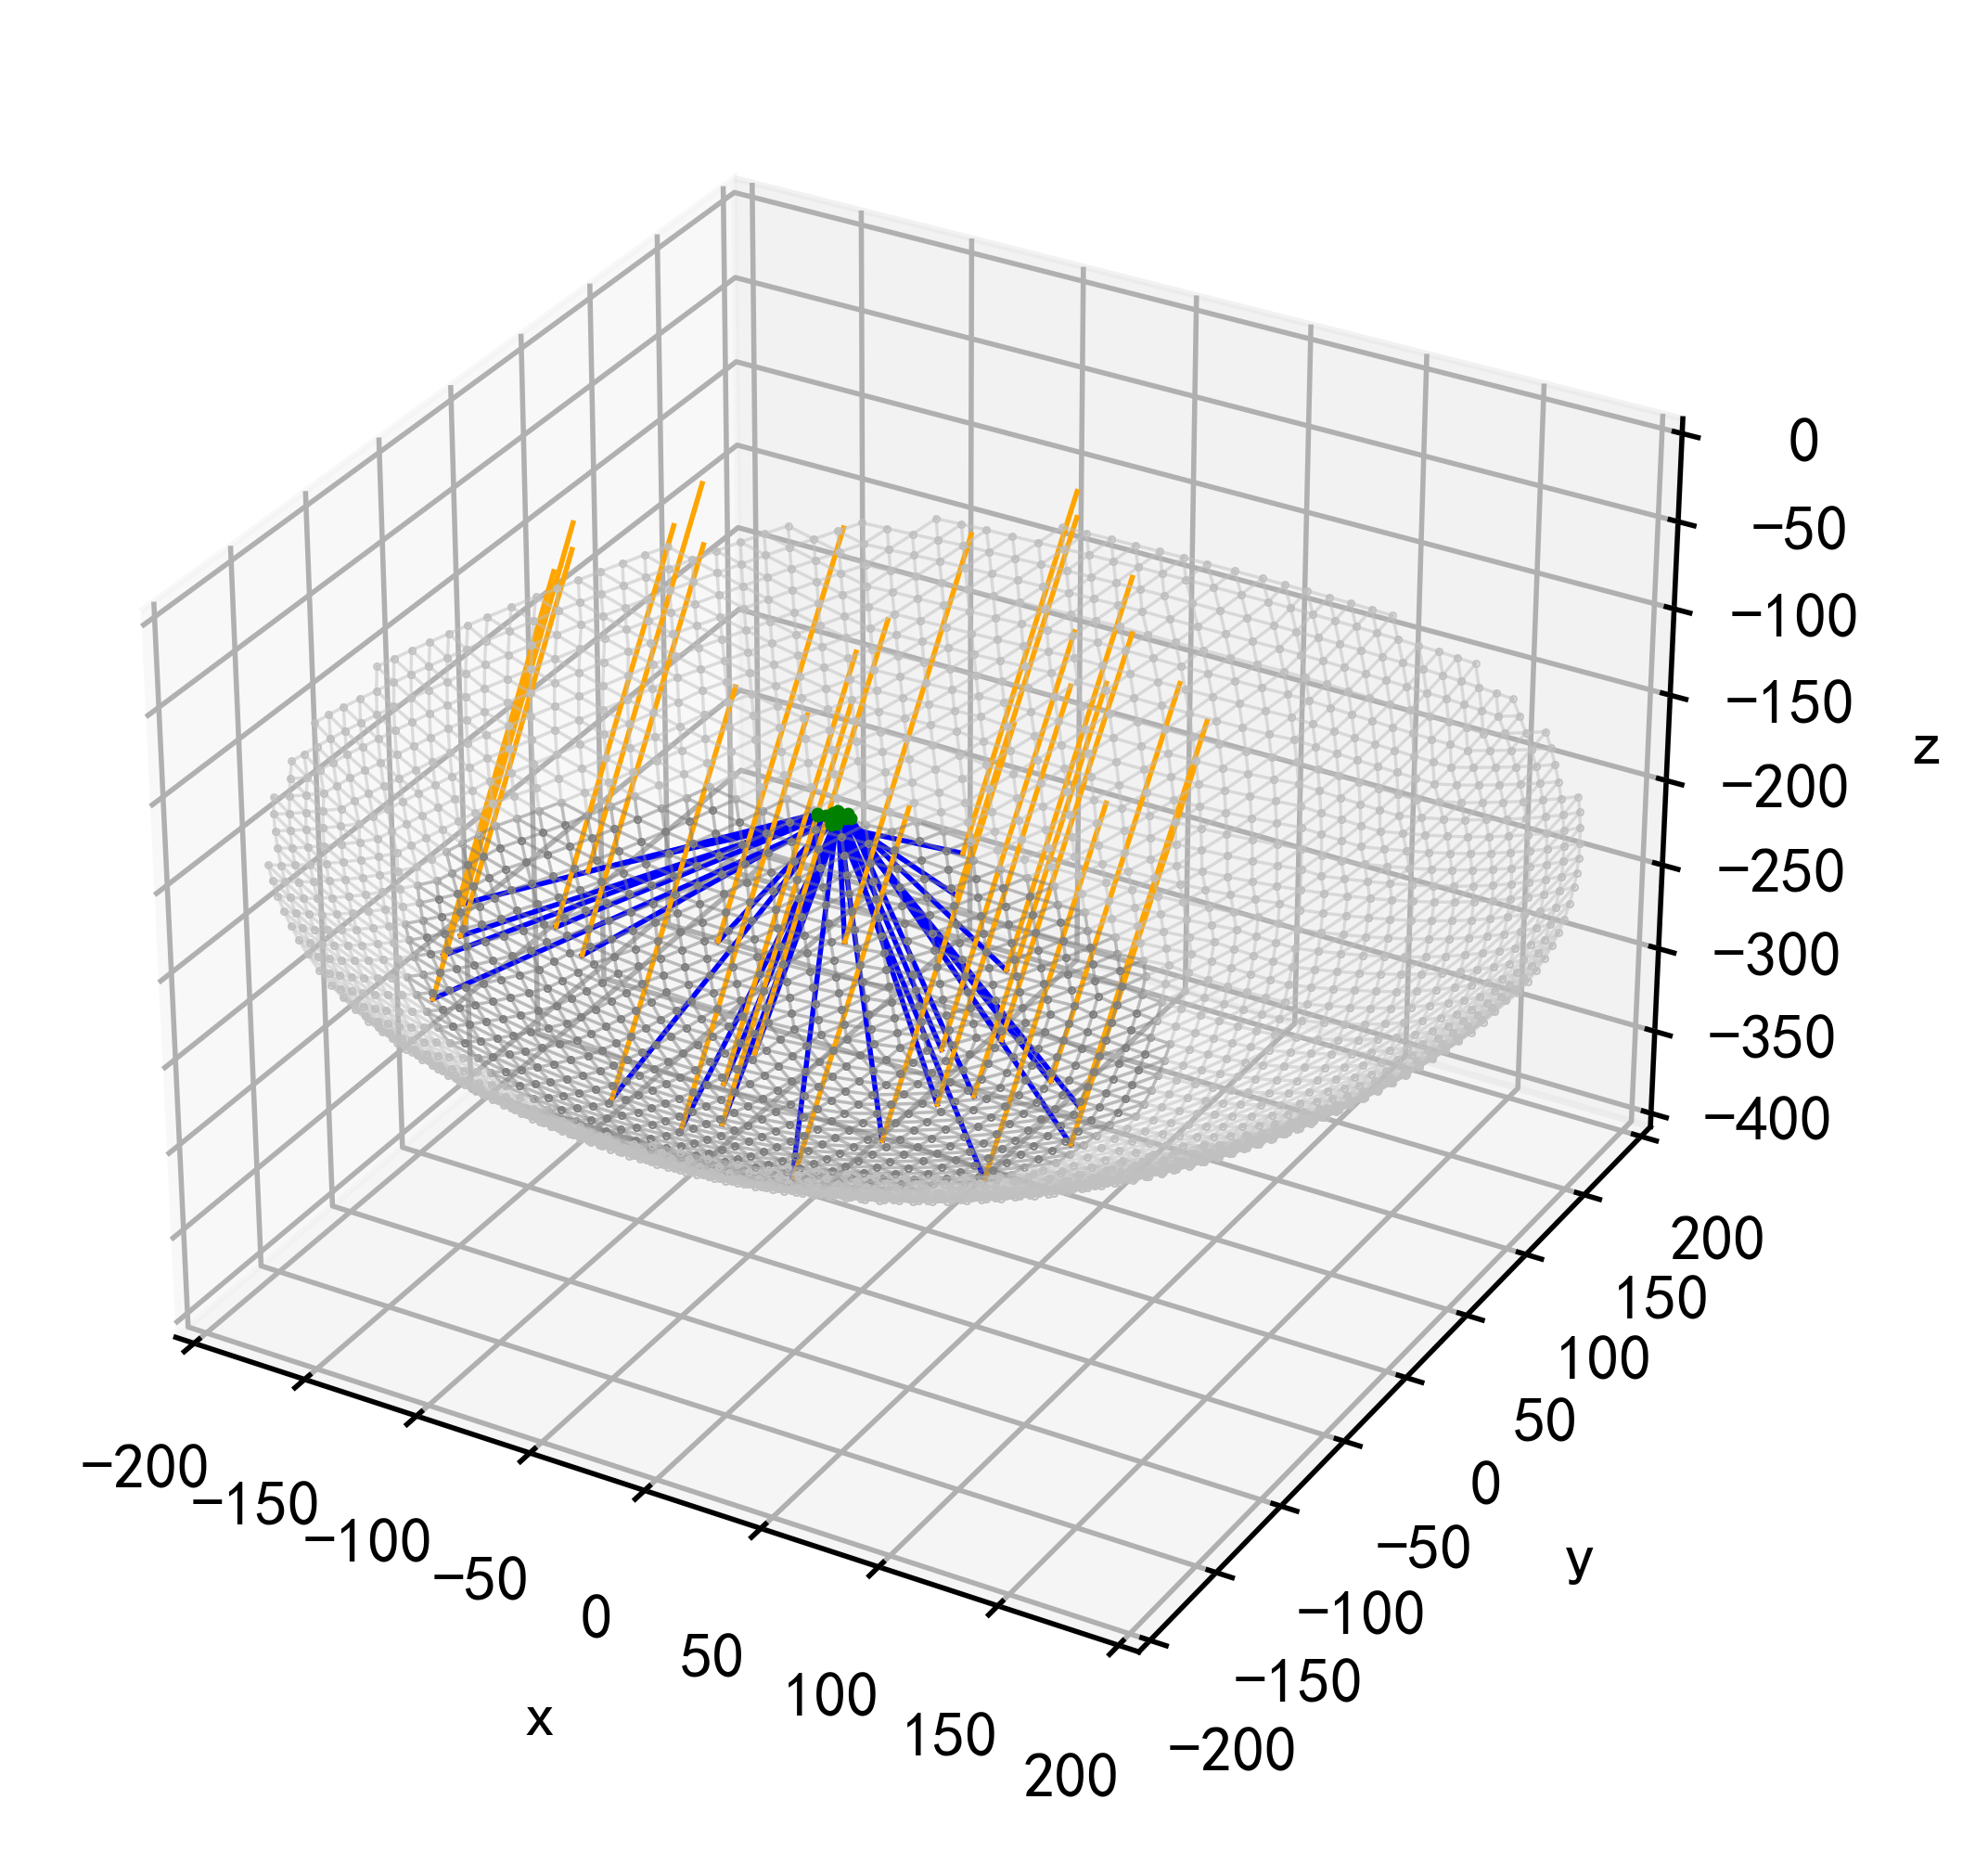
\includegraphics[width=1\textwidth]{rotate_reflect.png}
				\subcaption{光线反射图}
				\label{rotate_reflect}
			\end{minipage}
			\caption{问题2处理结果}
		\end{figure}

		图 \ref{rotate_diff} 反映了工作抛物面的形态放大 100 倍后的形态(原始位置加上一百倍的偏移量),可以发现除边缘外,内部凹陷,成抛物面形状。同时,图 \ref{rotate_diff} 分级表示了两个节点内的主索变化程度,从图中可以看出在工作抛物面的边缘区域以及底部主索变化程度较高。图 \ref{rotate_reflect} 模拟了光线照射的结果,黄线表示入射光,蓝线表示反射后的光,绿色点表示其穿过馈源舱所在平面的位置,可以发现绝大多数光线都被反射至馈源舱附近区域,结果符合预期。
		
		
	\section {问题三模型建立与求解}
	\subsection {模型建立}
	\subsubsection {信号的传播模型}
		天体S所发射的电磁波信号沿直线传播,经反射面板反射不损失,其传播示意图如图\ref {fig:reflection}所示。
		\begin{figure}[!h]
			\centering
			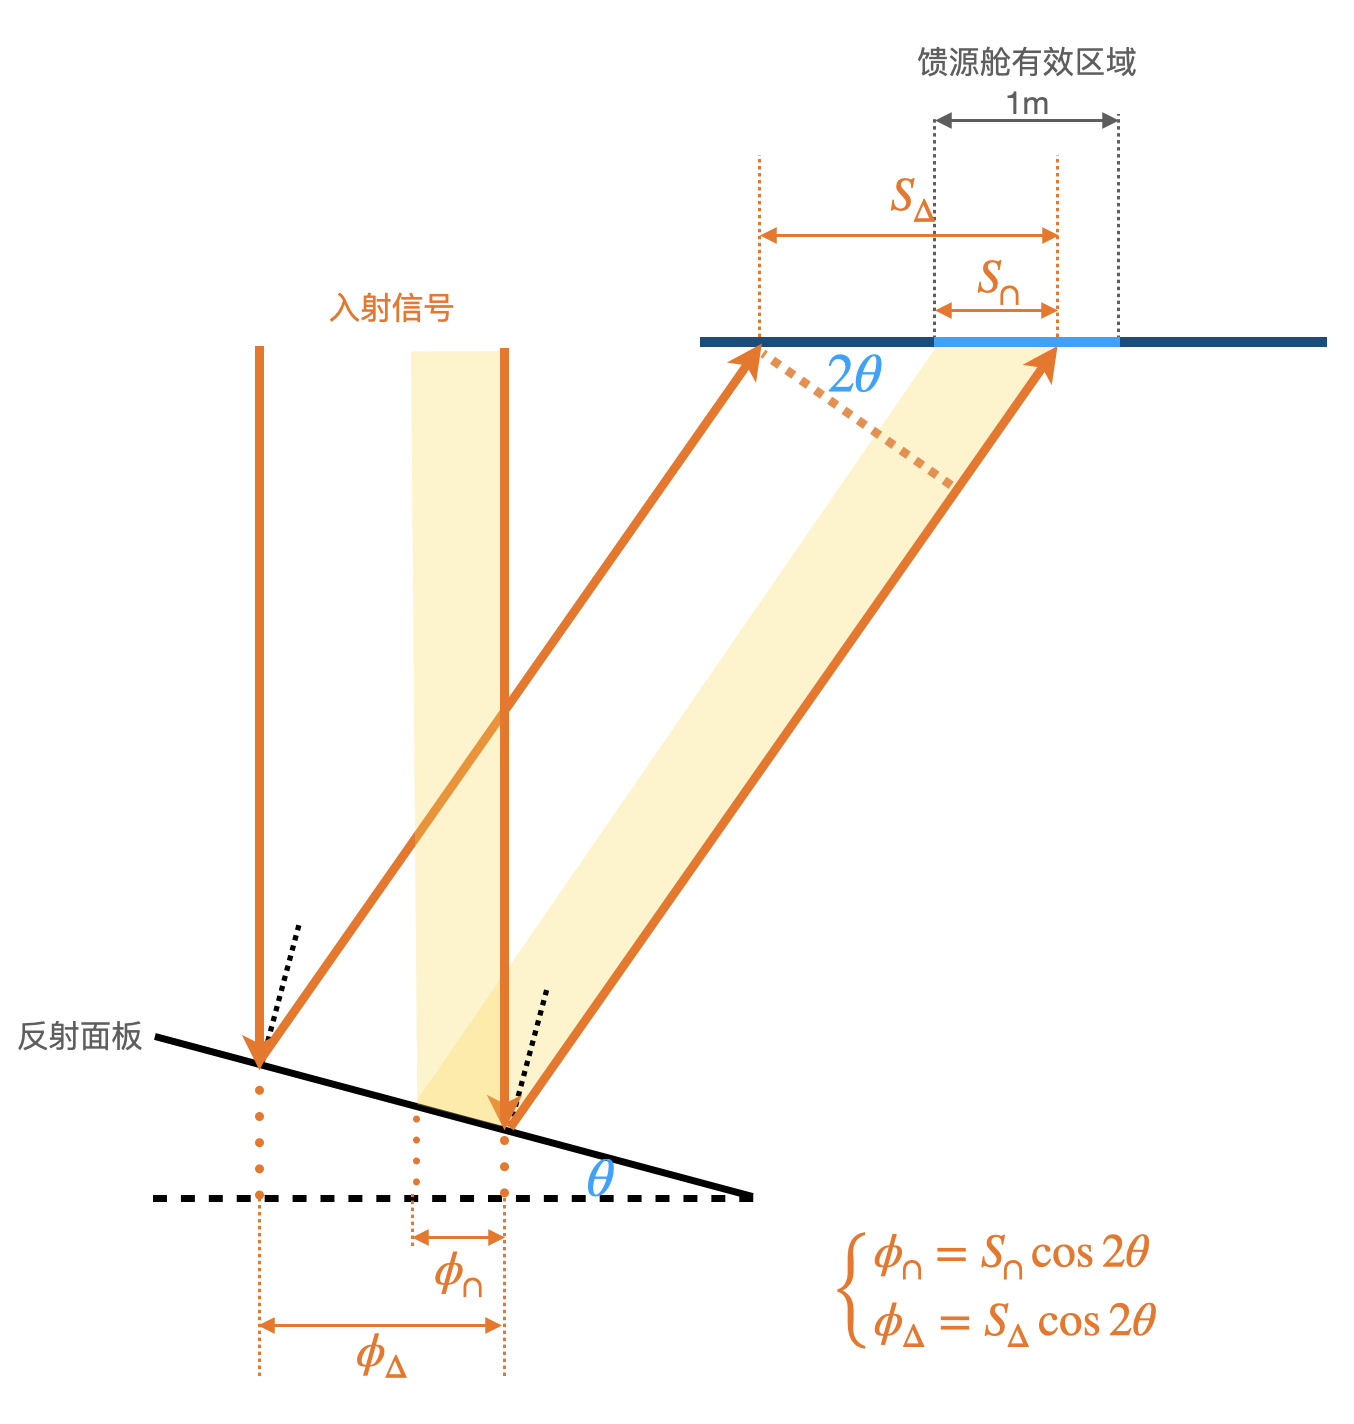
\includegraphics[height=0.4\textwidth]{reflection.png} % 表示缩放到文本行的 0.4 倍宽
			\caption{信号反射}
			\label{fig:reflection}
		\end{figure}
		考虑单块反射面板,假设入射信号在垂直于入射角度的平面上是均匀分布的,入射信号射入馈源舱有效接收区域的部分用淡黄色表示,入射信号平均分布在投影面积$\phi_\Delta$上,其中$\phi_\cap$的部分投射到馈源舱有效接收区域,称为接收面积,接收比为$\frac{\phi_\cap}{\phi_\Delta}$,记它们投射到馈源舱接收区域所在平面上的面积分别为$S_\Delta$,$S_\cap$,则有
		\begin{align}
			&\begin{cases}
				\phi_\Delta = S_\Delta\cos 2 \theta,\\
				\phi_\cap = S_\cap\cos 2 \theta,\\
			\end{cases}
		\end{align}
	
	
		故单块反射面板接收比为$\frac{\phi_\cap}{\phi_\Delta} = \frac{S_\cap}{S_\Delta}$。求整个抛物面反射面板接收比,应求组成反射抛物面的所有反射面板的接收面积之和与投影面积之和之比,即:
		\begin{equation}
			\eta = \frac{\sum_{i=1}^{m}\phi_\cap}{\sum_{i=1}^{m}\phi_\Delta} = \frac{\sum_{i=1}^{m}S_\cap \cos 2 \theta_i}{\sum_{i=1}^{m}S_\Delta \cos 2 \theta_i}
			\label{eq:receive_rate}
		\end{equation}
	
	\subsection	{模型求解}
	
		在问题二中,我们已解得最优理想抛物面形状,若我们忽略伸缩量不超过 $0.6m$ 和主索拉伸量不超过 $0.07\%$ 的约束条件,将所有主索节点移动至理想抛物面上并计算接收比,则理论上应得到实际接收比的上界,称之为理想抛物面接收比。为此,我们分别计算了实际反射平面形状、理想抛物面形状和基准球面形状情形下的接收比,结果如表\ref{tab:resultT3}所示。
		
		\begin{table}[!h]
			\centering
			\begin{tabular}{|l|l|l|}
				\hline
				实际接收比 & 理想抛物面接收比 & 球面接收比 \\ \hline
				1.137517\% & 1.175547\% & 0.861139\% \\ \hline
			\end{tabular}
			\caption{问题三结果}
			\label{tab:resultT3}
		\end{table}

	\section{模型评价与总结}
	\subsection{合理性分析}
	\subsubsection {接收比合理性}
		本小节中我们估计理论最佳接收比并与实际接收比进行比较,以验证模型结果的合理性。
		
		
		整个抛物面反射面板的接收比不大于单块反射面板接收比的最大值$\eta_{max}$,考虑由信号传播模型给出的接收比公式:
		\begin{equation*}
		  \begin{aligned}
		    \eta_k &= \frac{\phi_\cap}{\phi_\Delta} \\
		           &= \frac{S_\cap}{S_\Delta} \\
		      	   &= \frac{S_{rec} \cos 2 \theta}{S_{ref} \cos \theta}
		  \end{aligned}
		\end{equation*}
		其中$S_{rec}$表示馈源舱有效接收区域的面积,$S_{ref}$表示反射面板的面积。由于反射面板三边的变化范围均不大于$0.07\%$,可以采用边长的均值来参与估计,以边长为全体边长均值的等边三角形面积作为估计面积。考虑函数$f(\theta) = \frac{\cos 2 \theta}{\cos \theta} = 2\cos \theta - \frac{1}{\cos \theta}$,由于馈源舱照明区域口径为300m,近似认为其张角为120°,故$\theta \in (0, \pi/3]$,而$f(\theta)$在该区间内是单调递减的,所以$f(\theta) < f(0) = 1$。 
		等边三角形的边长取11.391m,代入计算得接收比估计值为1.398\% 。
		
		
		据此可以认为本文模型得出的结果是具有高合理性的。
		
		
	\subsection{馈源舱接收比与半径关系探索}
	
		实验中我们发现,众多反射信号会聚集在馈源舱附近,若略微增大馈源舱半径,其接收比将得到较大的提升。为此,我们定量计算了理想抛物面、实际反射平面和基准球面三种情形下馈源舱接收比与半径的关系,并以球面为基准求出相对接收比,如图\ref{fig:rate-p}所示。
		
		\begin{figure}[!h]
			\centering
			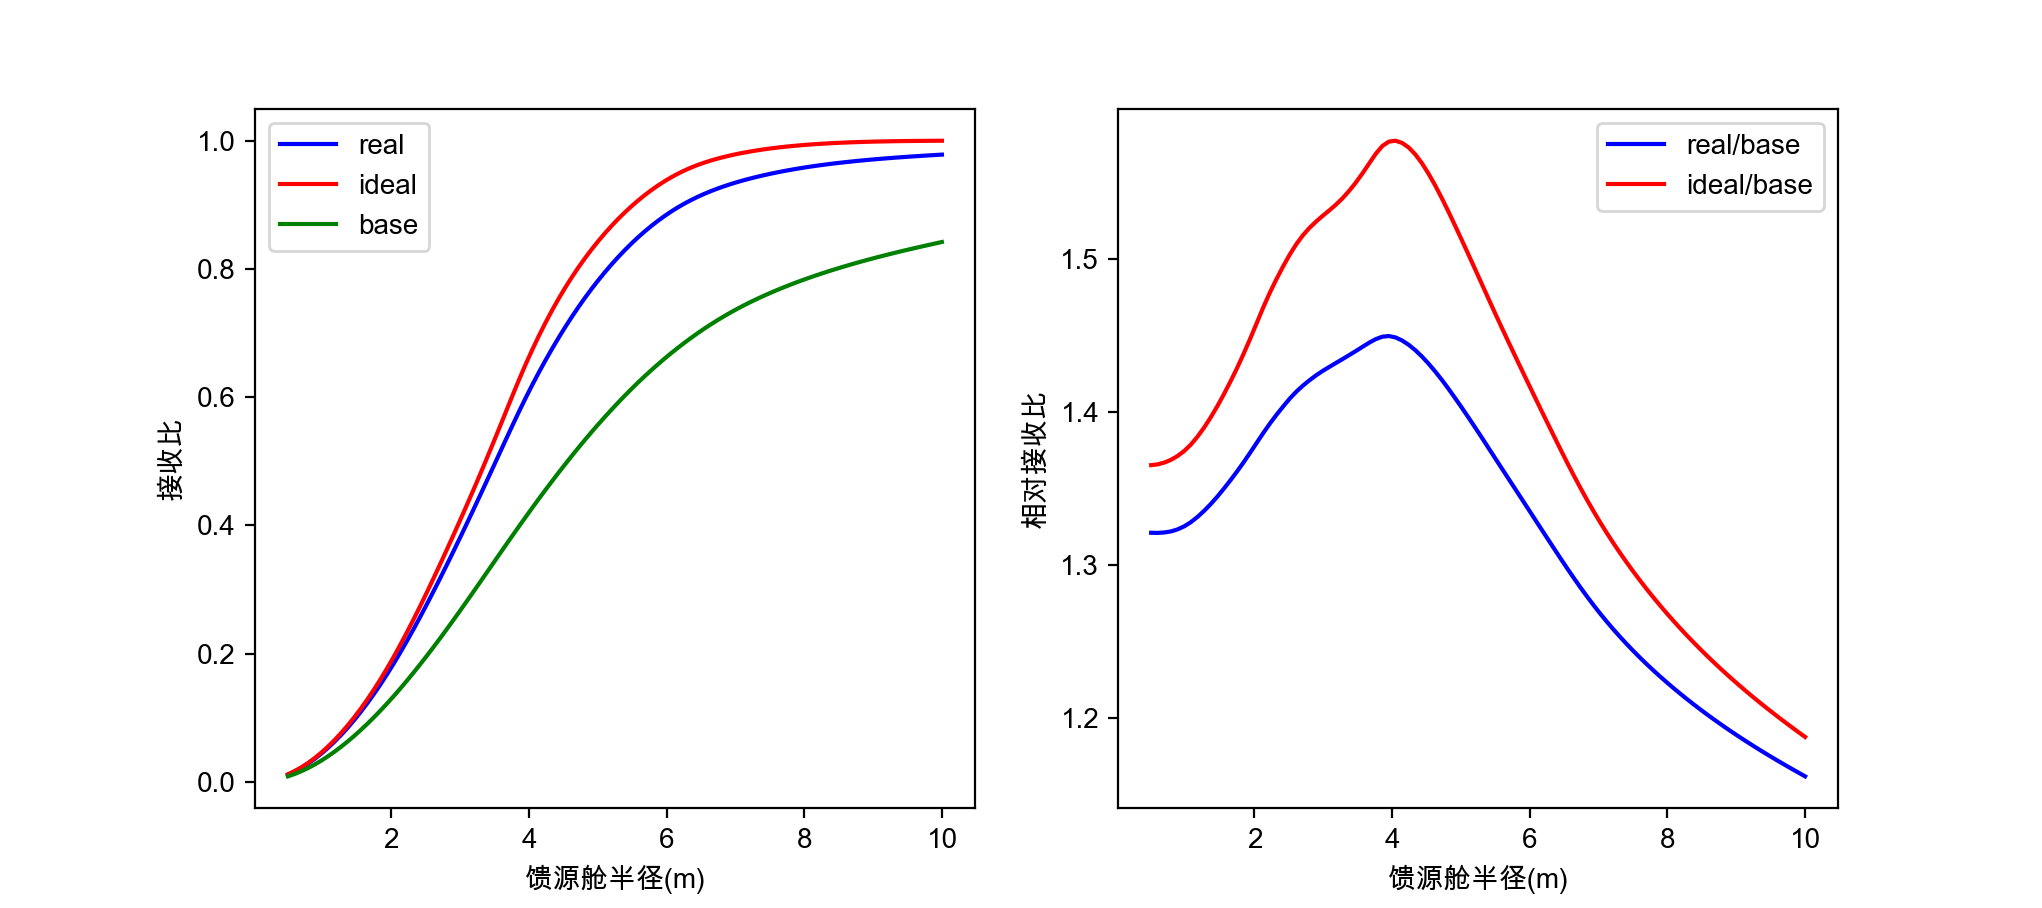
\includegraphics[height=0.4\textwidth]{rate-p.png} % 表示缩放到文本行的 0.4 倍宽
			\caption{馈源舱接收比与半径关系}
			\label{fig:rate-p}
		\end{figure}
	
		从图中可以发现,随着馈源舱半径的增大,接收比的增大率先增后减;同时,相对(基准球面)接收比在半径为 $4m$ 左右时达到顶峰。这指示我们,在当下如果我们能够克服其他困难增大馈源舱半径,我们能够获取巨大的接收比收益。

	
	\subsection{模型改进}
	\subsubsection {模型缺点}
		模型在分析FAST的索网控制策略时仅考虑了促动器的径向位移控制,而没有考虑力的作用以及其它现实因素如风速、降雨等对形成抛物面的控制策略的影响。
	\subsubsection {模型优化方向}
		当前模型由于规模较大,求解存在一定的困难,我们提出一个可能的优化的方向。在求解优化模型时,可以根据实时抛物面拟合情况,重新确定所需要的优化的节点个数,而不将所有参与形变的节点全部同时进行优化,否则不但效率降低,也可能影响算法的结果质量。具体的做法,可以采取优先调整对优化目标函数贡献最大的节点,也即径向误差最大的节点。由于主索存在变形幅度的限制,一个节点的径向误差过大势必连带其周围的节点,而对径向误差大的节点先调整,也会因主索变化幅度限制而对周围节点产生连带作用。因此优先调整对目标函数贡献最大的节点,在理论上能够对算法的效率做出提升。
		另一值得指出的点是,本文模型所采取的优化准则是将主索节点尽量控制在理想抛物面上,这也与所查阅的其它文献的准则相同。这种优化准则是否有可能并非全局最优的优化策略,而只是局部最优呢?例如,设计算法使反射面板尽可能与理想抛物面相切的优化准则所带来的效果如何,是否优于节点拟合抛物面,这些问题尚有待验证,却仍不失为一种优化本文模型的方向。
	\section{参考文献}
	
	\begin{thebibliography}{9}%宽度9
		\bibitem[1]{bib1}
		南仁东.
		\newblock 500m球反射面射电望远镜FAST\allowbreak[A]
		\newblock 中国科学G辑, 2005.
		\bibitem[2]{bib2}
		端素红.
		\newblock 基于粒子群优化算法的FAST整网控制策略研究
		\newblock 东北大学, 2015
		\bibitem[3]{bib3} 朱忠义等.
		\newblock 500m口径球面射电望远镜索网结构形态和受力分析
		\newblock 建筑结构学报. 2021
	\end{thebibliography}
	
		\newpage
	\section{附录}
	\begin{appendices}
	\section{节点数据处理}
	\begin{lstlisting}[language=python]
		# 用于模拟光线照射并计算吸收率
	import numpy as np
	import matplotlib.pyplot as plt
	from tqdm import tqdm
	from math import sin, cos, pi
	from mcm import paint
	
	R = 300.4
	k = 0.466
	target_z = -(1 - k) * R
	lim = 150 ** 2
	alpha = 36.795 / 180 * pi
	beta = 78.169 / 180 * pi
	
	
	def get_ideal_mu(p: float, c: float, ori_pos, mov_vec):
	    """
	    :param mov_vec: 移动向量
	    :param ori_pos: 原始点
	    :param p: 抛物面参数
	    :param c: 抛物面参数
	    :return: 主索节点按移动方向到抛物面上的移动距离
	    """
	    x0, y0, z0 = ori_pos[1:, 0], ori_pos[1:, 1], ori_pos[1:, 2]
	    i, j, kk = mov_vec[1:, 0], mov_vec[1:, 1], mov_vec[1:, 2]
	    Delta = (
	            (p ** 2) * (kk ** 2) + 2 * i * j * x0 * y0 + 2 * j * kk * p * y0 + 2 * i * kk * p * x0
	            - (j ** 2) * (x0 ** 2) - (i ** 2) * (y0 ** 2)
	            - 2 * p * z0 * (i ** 2) - 2 * p * z0 * (j ** 2)
	            - c * (i ** 2) - c * (j ** 2)
	    )
	    mu1 = (-(i * x0 + j * y0 + p * kk) + np.sqrt(Delta)) / (i ** 2 + j ** 2)
	    mu2 = (-(i * x0 + j * y0 + p * kk) - np.sqrt(Delta)) / (i ** 2 + j ** 2)
	    x0, y0, z0 = ori_pos[0]
	    i, j, kk = mov_vec[0]
	    mu1 = np.concatenate(([-(x0 ** 2 + y0 ** 2 + 2 * p * z0 + c) / (2 * p * kk)], mu1))
	    mu2 = np.concatenate(([-(x0 ** 2 + y0 ** 2 + 2 * p * z0 + c) / (2 * p * kk)], mu2))
	    mu1[np.fabs(mu1) > np.fabs(mu2)] = mu2[np.fabs(mu1) > np.fabs(mu2)]
	    return mu1
	
	
	def get_ideal_pos(p: float, c: float, ori_pos, mov_vec):
	    """
	    :param mov_vec: 移动向量
	    :param ori_pos: 原始点
	    :param p: 抛物面参数
	    :param c: 抛物面参数
	    :return: 主索节点按移动方向到抛物面上的移动距离
	    """
	    return ori_pos + get_ideal_mu.reshape(-1, 1) * mov_vec
	
	
	def generate_ray(A_tri, B_tri, C_tri, ray_rho, rseed):
	    """
	    :param A_tri: 顶点 A 坐标
	    :param B_tri: 顶点 B 坐标
	    :param C_tri: 顶点 C 坐标
	    :param ray_rho: 生成的光线密度
	    :param rseed: 随机数种子
	    :return: 生成的光线
	    """
	    np.random.seed(rseed)
	    A_tri, B_tri, C_tri = A_tri[:-1], B_tri[:-1], C_tri[:-1]
	    S_tri = np.fabs(
	        A_tri[0] * (B_tri[1] - C_tri[1]) + B_tri[0] * (C_tri[1] - A_tri[1]) + C_tri[0] * (A_tri[1] - B_tri[1]))
	    S_tri /= 2
	    # print(S_tri)
	
	    ray_num = int(S_tri * ray_rho)
	    # print(ray_num)
	    params = np.random.rand(ray_num, 3)
	    params = params / np.sum(params, axis=1).reshape(-1, 1)
	    aa, bb, gamma = params[:, 0].reshape(-1, 1), params[:, 1].reshape(-1, 1), params[:, 2].reshape(-1, 1)
	    return aa * A_tri + bb * B_tri + gamma * C_tri
	
	
	def reflact_ray(A_tri, B_tri, C_tri, ray):
	    """
	    :param A_tri: 三角形顶点 A
	    :param B_tri: 三角形顶点 B
	    :param C_tri: 三角形顶点 C
	    :param ray: 入射光线数组,ray[i] = [x, y] 表示第 i 条光线投影 xOy 平面坐标为 (x, y)
	    :return: 返回光线反射后的起始点以及向量
	    """
	    # 计算任意两个向量
	    u = A_tri - B_tri
	    v = B_tri - C_tri
	    # 计算法向量
	    # n1 = np.array([u[2] * v[1] - u[1] * v[2], u[0] * v[2] - u[2] * v[0], u[1] * v[0] - u[0] * v[1]])
	    n = np.cross(u, v)
	    # print(n)
	    # print(n1)
	    if n[2] < 0:
	        n = -n
	    d = -A_tri.dot(n)
	    # 计算光线在平面上的落点
	    z_ray = -(d + ray.dot(n[:2].reshape(-1, 1))) / n[2]
	    # print(ray)
	    # print(z_ray)
	    ray_point = np.concatenate((ray, z_ray), axis=1)
	    # 在光线上方取一点,并计算其对称点
	    point_above = ray_point.copy()
	    point_above[:, 2] += 1
	    point_below = point_above - 2 * np.abs(point_above.dot(n.reshape(-1, 1)) + d) / np.sum(n ** 2) * n
	    # 根据光线对称点与光线落点求出其反射向量
	    return ray_point, ray_point - point_below
	
	
	def verify_shoot(point, vector):
	    """
	    :param point: point[i] = [x, y, z] 表示光线的起点
	    :param vector: vector[i] = [a, b, c] 表示光线的方向向量
	    :return: verify[i] 表示第 i 束光线能否照射在馈源舱中
	    """
	    t = (target_z - point[:, -1]) / vector[:, -1]
	    final_point = point + t.reshape(-1, 1) * vector
	    # return (final_point[:, :-1] - np.zeros(shape=(1, 2))) ** 2 < 1
	    return np.sum(final_point[:, :-1] ** 2, axis=1) < 0.5 ** 2
	
	
	def check_tri_pos(tri_data, pos_data):
	    """
	    根据三角形的顶点序号,以及给定顶点的位置信息,返回三角形的顶点位置信息
	    :param tri_data: tri_data[i] = [x, y, z] 表示第 i 个三角形的三边顶点序号为 [x, y, z]
	    :param pos_data: pos_data[i] = [x, y, z] 表示第 i 个点的位置为 (x, y, z)
	    :return: 返回 tri_pos,tri_pos[i] = [A, B, C] 其中 A, B, C 为顶点坐标
	    """
	    return pos_data[tri_data]
	
	
	def check_all_pieces(all_tri):
	    rho = 0.05
	    seed = 3
	    all_num = 0
	    shoot_num = 0
	    all_ray_point = np.empty(shape=(0, 3))
	    all_ray_out = np.empty(shape=(0, 3))
	    valid_tri_num = 0
	    for e in tqdm(all_tri):
	        if e[0][0] ** 2 + e[0][1] ** 2 < lim and e[1][0] ** 2 + e[1][1] ** 2 < lim \
	                and e[2][0] ** 2 + e[2][1] ** 2 < lim:
	            valid_tri_num += 1
	            ray_down = generate_ray(e[0], e[1], e[2], rho, seed)
	            ray_point, ray_out = reflact_ray(e[0], e[1], e[2], ray_down)
	            all_ray_point = np.concatenate((all_ray_point, ray_point), axis=0)
	            all_ray_out = np.concatenate((all_ray_out, ray_out), axis=0)
	            all_num += ray_down.shape[0]
	            shoot_num += np.sum(verify_shoot(ray_point, ray_out))
	    print(valid_tri_num)
	    return shoot_num / all_num, all_ray_point, all_ray_out
	
	
	def rotate_all_point(ori_pos, d):
	    sa = sin(alpha)
	    ca = cos(alpha)
	    sb = sin(beta)
	    cb = cos(beta)
	    M0 = np.array([
	        [sa, -ca, 0],
	        [ca * sb, sa * sb, -cb],
	        [ca * cb, sa * cb, sb]
	    ]).T
	    if d == 1:
	        M0 = np.linalg.inv(M0)
	    return M0.dot(ori_pos.T).T
	
	
	def get_edges(tri_data, ori_data):
	    s = set()
	    for e in tri_data:
	        for i in range(3):
	            if np.sum(ori_data[e[i]][:2] ** 2) > lim or \
	                    np.sum(ori_data[e[(i + 1) % 3]][:2] ** 2) > lim:
	                continue
	            if e[i] > e[(i + 1) % 3]:
	                s.add((e[i], e[(i + 1) % 3]))
	            else:
	                s.add((e[(i + 1) % 3], e[i]))
	    lt = list(s)
	    return np.array(lt)
	
	
	def get_all_edges(tri_data, ori_data):
	    s = set()
	    for e in tri_data:
	        for i in range(3):
	            if e[i] > e[(i + 1) % 3]:
	                s.add((e[i], e[(i + 1) % 3]))
	            else:
	                s.add((e[(i + 1) % 3], e[i]))
	    lt = list(s)
	    return np.array(lt)
	
	
	def get_outter_edges(tri_data, ori_data):
	    s = set()
	    for e in tri_data:
	        for i in range(3):
	            if np.sum(ori_data[e[i]][:2] ** 2) > lim or \
	                    np.sum(ori_data[e[(i + 1) % 3]][:2] ** 2) > lim:
	                if e[i] > e[(i + 1) % 3]:
	                    s.add((e[i], e[(i + 1) % 3]))
	                else:
	                    s.add((e[(i + 1) % 3], e[i]))
	    lt = list(s)
	    return np.array(lt)
	
	
	# 用来绘制光线图
	def all_test_paint():
	    tri_datapath = "./data/tri.csv"
	    # pos_datapath = "./data/baby_mov_pos.csv"
	    ori_datapath = "./data/points.npy"
	    pos_datapath = "./data/final_p.npy"
	    # pos_data = np.load(pos_datapath)
	    pos_data = np.load(pos_datapath)
	    ori_data = np.load(ori_datapath)
	    tri_data = np.loadtxt(tri_datapath, delimiter=",", dtype=int)
	    tri_pos_data = check_tri_pos(tri_data, pos_data)
	    accept_rate, all_ray_point, all_ray_out = check_all_pieces(tri_pos_data)
	
	    inv = 500
	    ax = paint.get_ax()
	    paint.paint_light(all_ray_point, all_ray_out, inv, ax)
	    edges = get_edges(tri_data, pos_data)
	    outter_edges = get_outter_edges(tri_data, ori_data)
	    paint.paint_net(pos_data[edges], ax, np.full(shape=edges.shape[0], fill_value=10))
	    paint.paint_net(pos_data[outter_edges], ax, np.full(shape=outter_edges.shape[0], fill_value=9))
	    # paint.paint_receiver(ax)
	    plt.savefig("./figure/light_reflect.png", dpi=500, bbox_inches='tight')
	    plt.show()
	
	
	def diff_paint():
	    ori_data_path = "./data/final_p.npy"
	    new_data_path = "./data/best_pos_1.npy"
	    tri_data_path = "./data/tri.csv"
	    ori_data = np.load(ori_data_path)
	    new_data = np.load(new_data_path)
	    tri_data = np.loadtxt(tri_data_path, delimiter=",", dtype=int)
	
	    # valid_id = np.nonzero(np.sum(ori_data[:, :2]**2, axis=1) <= lim)[0]
	    # now_data = ori_data.copy()
	    # now_data[valid_id] = new_data
	    ax = paint.get_ax()
	    paint.paint_diff_net(get_all_edges(tri_data, ori_data), ori_data, new_data, 100, ax)
	    plt.savefig("./figure/diff_net.png", dpi=500, bbox_inches='tight')
	    plt.show()
	
	
	def for_pso():
	    tri_data_path_ = "./data/tri.csv"
	    ori_data_path_ = "./data/final_p.npy"
	    tri_data_ = np.loadtxt(tri_data_path_, delimiter=",", dtype=int)
	    ori_data_ = np.load(ori_data_path_)
	    valid_data = np.nonzero(np.sum(ori_data_[:, :2] ** 2, axis=1) <= lim)[0]
	    edges = get_edges(tri_data_, ori_data_)
	    np.save("./data/edges.npy", edges)
	    np.save("./data/valid.npy", valid_data)
	    # print(valid_data)
	
	
	def paint_incline():
	    tri_data_path = "./data/tri.csv"
	    tri_data = np.loadtxt(tri_data_path, delimiter=",", dtype=int)
	    ori_data = np.load("./data/final_p.npy")
	    # 得到在新坐标系中的坐标
	    right_data = np.load("./data/best_pos_2.npy")
	    # right_data = ori_data.copy()
	    # 映射到旧坐标系中倾斜的坐标
	    incline_data = rotate_all_point(right_data, -1)
	
	    # 得到在新坐标中散射的光线
	    tri_pos_data = check_tri_pos(tri_data, right_data)
	    accept_rate, all_ray_point, all_ray_out = check_all_pieces(tri_pos_data)
	    all_ray_com_point = np.concatenate((all_ray_point[:, :2],
	                                       np.full(fill_value=-50, shape=(all_ray_point.shape[0], 1))),
	                                       axis=1)
	    # 旋转至旧坐标系中
	    all_ray_com_point = rotate_all_point(all_ray_com_point, -1)
	    all_ray_point = rotate_all_point(all_ray_point, -1)
	    all_ray_out = rotate_all_point(all_ray_out, -1)
	
	    # 绘制图形
	    plt.rcParams['font.sans-serif'] = ['SimHei']  # 用来正常显示中文标签
	    plt.rcParams['axes.unicode_minus'] = False  # 用来正常显示负号
	    ax = paint.get_ax()
	
	    # 绘制参考线
	    # vec = -np.array([cos(beta) * cos(alpha), cos(beta) * sin(alpha), sin(beta)])
	    # ap = [0, 0, 0]
	    # bp = ap + R * vec
	    # ax.plot3D([ap[0], bp[0]], [ap[1], bp[1]], [ap[2], bp[2]], color="red")
	    # ax.plot3D([0, 0], [0, 0], [0, -R], color="green")
	
	    # 绘制在旧坐标中的光线映射
	    inv = 100
	    paint.paint_light_go(all_ray_point, all_ray_out, ax, inv)   # 离开的光线
	    paint.paint_lines(all_ray_point, all_ray_com_point, ax, inv)
	
	    # 绘制在坐标系下的坐标点
	    oori_data = rotate_all_point(ori_data, 1)
	    edges = get_edges(tri_data, oori_data)
	    outter_edges = get_outter_edges(tri_data, oori_data)
	    paint.paint_net(incline_data[edges], ax, np.full(shape=edges.shape[0], fill_value=10))
	    paint.paint_net(incline_data[outter_edges], ax, np.full(shape=outter_edges.shape[0], fill_value=9))
	    plt.savefig("./figure/rotate_reflect.png", dpi=500, bbox_inches='tight')
	
	    # 绘制在旧坐标中的差值图映射
	    ax = paint.get_ax()
	    edges = get_all_edges(tri_data, ori_data)
	    paint.paint_diff_net(edges, ori_data, incline_data, 100, ax)
	    plt.savefig("./figure/rotate_diff.png", dpi=500, bbox_inches='tight')
	
	    # ax = paint.get_ax()
	    # # paint.paint_diff_net(get_all_edges(tri_data, ori_data), ori_data, right_data, 1, ax)
	    # ax.scatter3D(ori_data[:, 0], ori_data[:, 1], ori_data[:, 2], s=0.3, color="orange")
	    # ax.scatter3D(right_data[:, 0], right_data[:, 1], right_data[:, 2], s=0.3, color="blue")
	
	
	if __name__ == "__main__":
	    # all_test_paint()
	    diff_paint()
	    # for_pso()
	    paint_incline()

	\end{lstlisting}
	\section{自定义绘图函数库}
	\begin{lstlisting} [language=python]
	# 用于模拟光线照射并计算吸收率
	import numpy as np
	import matplotlib.pyplot as plt
	from tqdm import tqdm
	from math import sin, cos, pi
	
	
	R = 300.4
	k = 0.466
	target_z = -(1 - k) * R
	lim = 150 ** 2
	
	
	def paint_net(edges, ax3d, drag):
	    colors = ["burlywood", "lightseagreen", "mediumseagreen", "darkseagreen", "goldenrod",
	              "darkorange", "orangered", "maroon", "mediumvioletred", "silver", "grey"]
	    for i in range(edges.shape[0]):
	        ax3d.plot3D(edges[i, :, 0], edges[i, :, 1], edges[i, :, 2], c=colors[drag[i]],
	                    lw=0.5, marker=".", markersize=0.5, alpha=0.5)
	
	
	def paint_receiver(ax3d):
	    x1 = np.linspace(-0.5, 0.5, 10)
	    y1 = np.sqrt(0.5**2 - x1**2)
	    y2 = -y1
	    y = np.concatenate((y1, y2, [y1[0]]))
	    x = np.concatenate((x1, x1, [x1[0]]))
	    z = np.full(shape=x.shape[0], fill_value=(k - 1)*R)
	    ax3d.plot3D(x, y, z, color="red")
	
	
	def paint_scatter_net(all_tri, ax3d):
	    ma = np.max(np.fabs(all_tri[:, :, 2]))
	    mi = np.min(np.fabs(all_tri[:, :, 2]))
	    all_tri = all_tri.reshape(-1, 3)
	    x, y, z = all_tri[:, 0], all_tri[:, 1], all_tri[:, 2]
	    cc = (np.fabs(z) - mi) / ma
	    for i in range(cc.shape[0]):
	        ax3d.scatter3D(x[i], y[i], z[i], c=[[cc[i] if cc[i] > 0.7 else 0.2,
	                                             cc[i] if cc[i] < 0.5 else 0.7, 0.25], ], s=1)
	
	
	def paint_light_down(ray_point, ax3d, interval):
	    for i in range(0, ray_point.shape[0], interval):
	        e = ray_point[i]
	        x = [e[0], e[0]]
	        y = [e[1], e[1]]
	        z = [-50, e[2]]
	        ax3d.plot3D(x, y, z, '-', color="orange", lw=0.8)
	
	
	def paint_light_with_angle(alpha, beta, ax3d):
	    point = np.zeros(3)
	    final_point = [cos(beta) * cos(alpha), cos(beta) * sin(alpha), sin(beta)]
	    final_point = -np.array(final_point) * R
	    x = [final_point[0], point[0]]
	    y = [final_point[1], point[1]]
	    z = [final_point[2], point[2]]
	    ax3d.plot3D(x, y, z, '-', color="orange")
	    point = rotate_all_point(alpha, beta, final_point.reshape(1, 3))
	    print(point)
	    x = point[:, 0]
	    y = point[:, 1]
	    z = point[:, 2]
	    ax3d.scatter3D(x, y, z, color="cornflowerblue")
	
	
	def paint_light_go(ray_point, ray_out, ax3d, interval):
	    n = ray_point.shape[0]
	    t = (target_z - ray_point[:, -1]) / ray_out[:, -1]
	    final_point = ray_point + t.reshape(-1, 1) * ray_out
	    print(np.sum(np.sqrt(np.sum(final_point[:, :-1] ** 2, axis=1)) < 0.5) / final_point.shape[0])
	    # ax3d.scatter(final_point[:, 0], final_point[:, 1], final_point[:, 2], color="green", s=1)
	    # print(ray_point, final_point)
	    for i in range(0, n, interval):
	        ax3d.scatter3D(final_point[i][0], final_point[i][1], final_point[i][2], color="green", s=1)
	        x = [ray_point[i][0], final_point[i][0]]
	        y = [ray_point[i][1], final_point[i][1]]
	        z = [ray_point[i][2], final_point[i][2]]
	        ax3d.plot3D(x, y, z, '-', color="blue", lw=0.8)
	
	
	def paint_lines(point_a, point_b, ax, interval):
	    for i in range(0, point_a.shape[0], interval):                     # 射入的光线
	        x = [point_a[i][0], point_b[i][0]]
	        y = [point_a[i][1], point_b[i][1]]
	        z = [point_a[i][2], point_b[i][2]]
	        ax.plot3D(x, y, z, '-', color="orange", lw=0.8)
	
	
	# 给定三角形数据以及各点位置,绘制光线照射图
	def paint_light(all_ray_point, all_ray_out, inv, ax):
	    paint_light_down(all_ray_point, ax, inv)
	    paint_light_go(all_ray_point, all_ray_out, ax, inv)
	
	
	def get_ax():
	    ax = plt.subplot(projection="3d")
	    ax.set_facecolor("white")
	    ax.set_xlim(-200, 200)
	    ax.set_ylim(-200, 200)
	    ax.set_zlim(-400, 0)
	    ax.set_xlabel("x")
	    ax.set_ylabel("y")
	    ax.set_zlabel("z")
	    return ax
	
	
	def paint_diff_net(edges, ori_data, new_data, N, ax):
	    # 计算拉力分级
	    tri_pos_new_data = new_data[edges]
	    tri_pos_old_data = ori_data[edges]
	    drag = np.zeros(tri_pos_old_data.shape[0])
	    for i in range(tri_pos_old_data.shape[0]):
	        new_dis = np.sqrt(np.sum((tri_pos_new_data[i][0] - tri_pos_new_data[i][1])**2))
	        old_dis = np.sqrt(np.sum((tri_pos_old_data[i][0] - tri_pos_old_data[i][1])**2))
	        drag[i] = np.fabs((old_dis - new_dis))/old_dis*100
	    dmax = np.max(np.fabs(drag))
	    dmin = np.min(np.fabs(drag))
	    if dmax != dmin:
	        drag = (np.fabs(drag) - dmin)/(dmax - dmin)*9
	    drag = np.int64(drag)
	    drag[drag >= 9] = 8
	    # 扩大相差距离
	    new_data[:, 2] = N * (new_data[:, 2] - ori_data[:, 2]) + ori_data[:, 2]
	    tri_pos_new_data = new_data[edges]
	    paint_net(tri_pos_new_data, ax, drag)
	\end{lstlisting}

	\section{计算相邻节点}
	\begin{lstlisting}[language=python]
	import numpy as np
	import pandas as pd
	
	
	def readdata(path):
	    df = pd.read_csv(path)
	    return np.array(df.iloc[:, 1:])
	
	
	# 输入三角形数据
	# 输出 adj[i] = [u, v]
	def get_adj(data_tri):
	    n, m = data_tri.shape
	    s = set()
	    for i in range(n):
	        for j in range(m):
	            s.insert((data_tri[i, j], data_tri[i, (j+1) % m]))
	    adj = np.zeros(len(s), 2)
	    for i, e in enumerate(s):
	        adj[i] = e
	    return adj
	
	
	# 输入所有点的坐标
	# 输出 dis[i] = [u, v, dis_uv]
	def get_dis(data_adj, data_pos):
	    dis = data_pos[data_adj[:, 0]] - data_pos[data_adj[:, 1]]
	    dis = np.square(dis)
	    dis = np.sqrt(np.sum(dis, axis=1))
	    return np.concatenate(data_adj, axis=1)
	
	
	def save_dis(file_tri, file_pos, file_dis):
	    data_tri = np.load(file_tri)
	    data_pos = np.load(file_pos)
	    data_adj = get_adj(data_tri)
	    data_dis = get_dis(data_adj, data_pos)
	    np.save(file_dis, data_dis)
	
	
	if __name__ == "__main__":
	    file_tri_ = "./distance/map3.npy"
	    file_pos_ = "./distance/map1.npy"
	    file_dis_ = "./distance/adj_dis.npy"
	    save_dis(file_tri_, file_pos_, file_dis_)

	\end{lstlisting}

		\section{检查数据与预处理}
	
	\begin{lstlisting}[language=python]
		import numpy as np
		import matplotlib.pyplot as plt
		from sklearn.metrics.pairwise import cosine_similarity
		plt.rcParams['font.sans-serif'] = ['Arial Unicode MS']
		plt.rcParams['axes.unicode_minus'] = False
		
		from readdata import get_final_data, get_map_data, get_dis_pairs, get_adj_pairs, get_ori_data, get_movable_ids
		from constant import const
		
		
		def check_for_on_sphere():
		suo = get_map_data(1)
		abserr = np.fabs((300.4 ** 2) - (suo ** 2).sum(axis=1))
		print(abserr)
		
		
		def check_for_alignment():
		mapping = {d[0]: i for i, d in enumerate(get_ori_data(1).to_numpy())}
		inv_mapping = {v: k for k, v in mapping.items()}
		
		suo = get_map_data(1)  # 主索节点坐标
		xia = get_map_data(2)[:, :3]  # 下端点坐标
		shang = get_map_data(2)[:, 3:]  # 上端点坐标
		v1 = shang - xia
		v2 = suo - shang
		v3 = suo - xia
		vo = -suo
		cos_sim1o = np.diagonal(cosine_similarity(v1, vo))
		cos_sim2o = np.diagonal(cosine_similarity(v2, vo))
		cos_sim3o = np.diagonal(cosine_similarity(v3, vo))
		print(np.min(cos_sim1o))
		print(np.min(cos_sim2o))
		print(np.min(cos_sim3o))
		print(np.argsort(cos_sim1o)[:10])
		print(np.argsort(cos_sim2o)[:10])
		print(np.argsort(cos_sim3o)[:10])
		
		abnorm_id = np.argsort(cos_sim2o)[:10]
		cos_sim = np.sort(cos_sim2o)
		print(np.arccos(cos_sim[:10]) * 180 / np.pi)
		print([inv_mapping[idx] for idx in abnorm_id])
		
		plt.scatter(suo[:, 0], suo[:, 1], s=1, label='normal')
		plt.scatter(suo[abnorm_id, 0], suo[abnorm_id, 1], color='r', s=4, label='abnormal')
		plt.axis('equal')
		plt.xlabel('$x(m)$')
		plt.ylabel('$y(m)$')
		plt.title('主索节点 $x-y$ 投影图')
		plt.legend()
		plt.show()
		
		
		def plot_data_on_xy(data, ax, title='', label=''):
		ax.scatter(data[:, 0], data[:, 1], s=1, label=label)
		ax.axis('equal')
		ax.set_xlabel('$x(m)$')
		ax.set_ylabel('$y(m)$')
		ax.set_title(title)
		ax.legend()
		
		
		def plot_xy():
		suo = get_map_data(1)  # 主索节点坐标
		xia = get_map_data(2)[:, :3]  # 下端点坐标
		shang = get_map_data(2)[:, 3:]  # 上端点坐标
		fig, ax = plt.subplots(1, 3)
		plot_data_on_xy(suo, ax[0], '主索节点 $x-y$ 投影图')
		plot_data_on_xy(xia, ax[1], '促动器下端点 $x-y$ 投影图')
		plot_data_on_xy(shang, ax[2], '基准态促动器上端点 $x-y$ 投影图')
		plt.show()
		
		
		def check_final_data():
		p, v = get_final_data(1)
		assert p.shape == v.shape == (const.n_points, 3)
		adj_pairs = get_adj_pairs()
		minsim = 1
		for i in range(len(p)):
		x, y = np.nonzero(adj_pairs == i)
		y = 1 - y
		minsim = min(minsim, (np.min(cosine_similarity(v[i:i+1], v[adj_pairs[x, y]]))))
		print(minsim)
		
		
		def check_distance_to_center():
		p, v = get_final_data(1)
		assert p.shape == v.shape == (const.n_points, 3)
		dists = np.sum(p[:, :2] ** 2, axis=1)
		# dists = p[:, 2]
		fig, ax = plt.subplots(1, 1)
		ax.scatter(np.arange(const.n_points), dists, s=4)
		plt.show()
		
		
		def calc_adj_theta():
		adj_pairs = get_adj_pairs()
		p, v = get_final_data(1)
		hudu, du = [], []
		dis = []
		for adj in adj_pairs:
		cossim = cosine_similarity(v[adj[0]].reshape(1, -1),
		v[adj[1]].reshape(1, -1))[0, 0]
		hudu.append(np.arccos(cossim))
		du.append(np.arccos(cossim) * 180 / np.pi)
		dis.append(np.linalg.norm(p[adj[0]] - p[adj[1]]))
		hudu, du = np.array(hudu), np.array(du)
		dis = np.array(dis)
		print(hudu.mean(), hudu.std(), np.max(hudu), np.min(hudu))
		print(du.mean(), du.std(), np.max(du), np.min(du))
		print(dis.mean(), dis.std(), np.max(dis), np.min(dis))
		# 结论:
		# 相邻节点伸缩方向 0.03 +- 0.0025 弧度,最大 0.0557 弧度
		# 相邻节点伸缩方向 2.17 +- 0.1439 度,最大 3.19 度
		# 相邻节点距离 11.391 +- 0.728 m
		
		
		def check_pairs():
		p, v = get_final_data(1)
		adj_pairs = get_adj_pairs()
		dis_pairs = get_dis_pairs(p)
		print(np.all(adj_pairs == dis_pairs[:, :2]))
		p, v = get_final_data(2)
		dis_pairs = get_dis_pairs(p)
		print(np.all(adj_pairs == dis_pairs[:, :2]))
		
		
		def check_coor_rotate():
		orip, oriv = get_final_data(1)
		rotp, rotv = get_final_data(2)
		print('rotate max error:', np.max(np.fabs((const.M @ orip.T).T - rotp)))
		print('rotate max error:', np.max(np.fabs((const.M @ oriv.T).T - rotv)))
		print('inverse rotate max error:', np.max(np.fabs((np.linalg.inv(const.M) @ rotp.T).T - orip)))
		print('inverse rotate max error:', np.max(np.fabs((np.linalg.inv(const.M) @ rotv.T).T - oriv)))
		
		
		def plot_curve():
		fig, ax = plt.subplots(1, 3)
		xrange = np.linspace(-100, 100, 100)
		circ = -np.sqrt((const.R ** 2 - xrange ** 2))
		p = np.array([-283, -280, -277])
		c = 2 * (const.R - const.F) * p - p * p
		for i in range(3):
		ax[i].plot(xrange, circ, c='grey', label='球面截面')
		ax[i].plot(xrange, (-c[i]-xrange**2)/p[i]/2, label='理想抛物面截面')
		ax[i].set_title('p=%f' % p[i])
		ax[i].set_xlabel('$x(m)$')
		ax[i].set_ylabel('$z(m)$')
		ax[i].axis('equal')
		ax[i].legend()
		plt.show()
		
		
		def check_result():
		import pandas as pd
		res1 = pd.read_csv('./result/result1.csv', header=None)
		res2 = pd.read_csv('./result/result2.csv', header=None)
		res3 = pd.read_csv('./result/result3.csv', header=None)
		
		dingdian = res1.to_numpy()
		print((const.M @ dingdian.T).T)
		
		jiedian = res2.to_numpy()
		mapping = {d[0]: i for i, d in enumerate(get_ori_data(1).to_numpy())}
		inv_mapping = {v: k for k, v in mapping.items()}
		print((get_movable_ids(2) == np.array([mapping[i[0]] for i in jiedian])).all())
		np.load('./result/quadratic/T2/best_pos.npy')
		
		
		if __name__ == '__main__':
		check_result()
		
	\end{lstlisting}
	
	\begin{lstlisting}[language=python]
		import numpy as np
		import matplotlib.pyplot as plt
		plt.rcParams['font.sans-serif'] = ['Arial Unicode MS']
		plt.rcParams['axes.unicode_minus'] = False
		
		from readdata import get_ori_data, get_map_data, get_final_data
		from constant import const
		
		mapping = {d[0]: i for i, d in enumerate(get_ori_data(1).to_numpy())}
		inv_mapping = {v: k for k, v in mapping.items()}
		
		from matplotlib import colors as mcolors
		colors = dict(mcolors.BASE_COLORS, **mcolors.CSS4_COLORS)
		by_hsv = sorted((tuple(mcolors.rgb_to_hsv(mcolors.to_rgba(color)[:3])), name)
		for name, color in colors.items())
		sorted_names = [name for hsv, name in by_hsv]
		
		
		def show_layers():
		data = get_ori_data(1).to_numpy()
		layers = []
		last_char = 'E'
		for d in data:
		if last_char == 'E' and d[0][0] == 'A':
		layers.append([])
		layers[-1].append(d[1:].astype(float))
		last_char = d[0][0]
		
		fig = plt.figure()
		ax = fig.add_subplot(111, projection='3d')
		for i, layer in enumerate(layers):
		pos = np.array(layer)
		ax.scatter(pos[:, 0], pos[:, 1], pos[:, 2],
		s=4, c=colors[sorted_names[i*5]], label='layer %d' % i)
		ax.set_xlim(-250, 250)
		ax.set_ylim(-250, 250)
		ax.set_zlim(-400, 0)
		ax.set_xlabel('$x(m)$')
		ax.set_ylabel('$y(m)$')
		ax.set_zlabel('$z(m)$')
		ax.set_title('数据的分层特征')
		plt.show()
		
		
		def show_groups():
		data = get_ori_data(1).to_numpy()
		p, v = get_final_data(1)
		groupA = np.array([mapping[data[i, 0]] for i in range(const.n_points) if data[i, 0][0] == 'A'])
		groupB = np.array([mapping[data[i, 0]] for i in range(const.n_points) if data[i, 0][0] == 'B'])
		groupC = np.array([mapping[data[i, 0]] for i in range(const.n_points) if data[i, 0][0] == 'C'])
		groupD = np.array([mapping[data[i, 0]] for i in range(const.n_points) if data[i, 0][0] == 'D'])
		groupE = np.array([mapping[data[i, 0]] for i in range(const.n_points) if data[i, 0][0] == 'E'])
		
		fig = plt.figure()
		ax = fig.add_subplot(111, projection='3d')
		ax.scatter(p[groupA, 0], p[groupA, 1], p[groupA, 2], s=4, c='r', label='A')
		ax.scatter(p[groupB, 0], p[groupB, 1], p[groupB, 2], s=4, c='g', label='B')
		ax.scatter(p[groupC, 0], p[groupC, 1], p[groupC, 2], s=4, c='b', label='C')
		ax.scatter(p[groupD, 0], p[groupD, 1], p[groupD, 2], s=4, c='orange', label='D')
		ax.scatter(p[groupE, 0], p[groupE, 1], p[groupE, 2], s=4, c='purple', label='E')
		ax.set_xlim(-250, 250)
		ax.set_ylim(-250, 250)
		ax.set_zlim(-400, 0)
		ax.set_xlabel('$x(m)$')
		ax.set_ylabel('$y(m)$')
		ax.set_zlabel('$z(m)$')
		ax.set_title('数据的分区特征')
		ax.legend()
		plt.show()
		
		
		def gen_mapping_data(save=False):
		data1 = get_ori_data(1).to_numpy()
		data2 = get_ori_data(2).to_numpy()
		data3 = get_ori_data(3).to_numpy()
		data1 = data1[:, 1:]
		data2 = data2[:, 1:]
		data3 = np.array([
		[mapping[data3[i, 0]],
		mapping[data3[i, 1]],
		mapping[data3[i, 2]]]
		for i in range(len(data3))])
		if save:
		np.save('map1.npy', data1.astype(float))
		np.save('map2.npy', data2.astype(float))
		np.save('map3.npy', data3.astype(int))
		print(data1)
		print(data2)
		print(data3)
		
		
		def gen_adj_pairs(save=False):
		"""
		:return: (n, 2), each row contain a pair of adjacent points
		"""
		data_tri = get_map_data(3)
		n, m = data_tri.shape
		s = set()
		for i in range(n):
		for j in range(m):
		u = data_tri[i, j]
		v = data_tri[i, (j+1) % m]
		s.add((min(u, v), max(u, v)))
		adj_pairs = np.array([list(e) for e in s])
		if save:
		np.save('adj_pairs.npy', adj_pairs)
		print(adj_pairs)
		
		
		def gen_final_data(save=False):
		coo = get_map_data(1)
		xia = get_map_data(2)[:, :3]
		shang = get_map_data(2)[:, 3:]
		v = shang - xia
		v = v / np.linalg.norm(v, axis=1).reshape(-1, 1)
		if save:
		np.save('final_p.npy', coo)
		np.save('final_v.npy', v)
		print(coo)
		print(v)
		
		
		if __name__ == '__main__':
		show_groups()
		
	\end{lstlisting}
	
	\begin{lstlisting}[language=python]
		import numpy as np
		
		
		def rotate_matrix(alpha, beta):
		sa = np.sin(alpha)
		ca = np.cos(alpha)
		sb = np.sin(beta)
		cb = np.cos(beta)
		M = np.array([
		[sa, -ca, 0],
		[ca*sb, sa*sb, -cb],
		[ca*cb, sa*cb, sb]
		]).T
		M = np.linalg.inv(M)
		return M
		
		
		class const:
		R = 300.4  # 球面半径
		D = 500  # 球面口径
		n_points = 2226
		n_edges = 6525
		n_faces = 4300
		F = 0.466 * R  # 两球面半径差
		r_receiver = 0.5  # 馈源舱接收半径
		d_parab = 300  # 抛物面口径
		rangep = (2*(R-F-301), 2*(R-F-299.8))  # 参数 p 理论范围(实际取 [-285, -275])
		alpha = 36.795 / 180 * np.pi
		beta = 78.169 / 180 * np.pi
		
		M = rotate_matrix(alpha, beta)  # 坐标变换矩阵
		
	\end{lstlisting}
	
	\begin{lstlisting}[language=python]
		import pandas as pd
		import numpy as np
		
		from constant import const
		
		
		def get_ori_data(i: int):
		return pd.read_csv('./data/%d.csv' % i, encoding='GBK')
		
		
		def get_map_data(i: int):
		return np.load('./data/map%d.npy' % i)
		
		
		def get_adj_pairs():
		return np.load('./data/adj_pairs.npy')
		
		
		def get_movable_ids(t_number: int):
		base_pos, v = get_final_data(t_number)
		movable_mask = np.sum(base_pos[:, :2] ** 2, axis=1) <= (150 ** 2)
		movable_ids = np.arange(const.n_points)[movable_mask]
		return movable_ids
		
		
		def get_layers():
		mapping = {d[0]: i for i, d in enumerate(get_ori_data(1).to_numpy())}
		data = get_ori_data(1).to_numpy()
		layers = []
		last_char = 'E'
		for i, d in enumerate(data):
		if last_char == 'E' and d[0][0] == 'A':
		layers.append([])
		layers[-1].append(mapping[d[0]])
		last_char = d[0][0]
		return layers
		
		
		def get_final_data(t: int):
		if t == 1:
		p = np.load('./data/final_p.npy')
		v = np.load('./data/final_v.npy')
		else:
		p = np.load('./data/final_p2.npy')
		v = np.load('./data/final_v2.npy')
		assert p.shape == v.shape == (const.n_points, 3)
		return p, v
		
		
		def get_dis_pairs(pos: np.ndarray):
		"""
		:param pos: (n, 3), 主索节点移动后的坐标
		:return: (k, 3), 相邻节点之间的距离, [i, j, dis_ij]
		"""
		adj_pairs = get_adj_pairs()
		assert adj_pairs.shape == (const.n_edges, 2)
		dis = pos[adj_pairs[:, 0]] - pos[adj_pairs[:, 1]]
		dis = np.linalg.norm(dis, axis=1)
		res = np.concatenate((adj_pairs, dis.reshape(-1, 1)), axis=1)
		assert res.shape == (const.n_edges, 3)
		return res
		
		
		def get_ideal_pos(p: float, base_pos: np.ndarray, v: np.ndarray):
		"""
		:param p: 抛物面参数
		:param base_pos: 基准面坐标
		:param v: 主索节点方向向量
		:return: 主索节点按移动方向到抛物面上的移动距离,及移动后的坐标
		"""
		c = - p * p + 2 * (const.R - const.F) * p
		x0, y0, z0 = base_pos[1:, 0], base_pos[1:, 1], base_pos[1:, 2]
		i, j, k = v[1:, 0], v[1:, 1], v[1:, 2]
		Delta = (
		(p**2)*(k**2) + 2*i*j*x0*y0 + 2*j*k*p*y0 + 2*i*k*p*x0
		- (j**2)*(x0**2) - (i**2)*(y0**2)
		- 2*p*z0*(i**2) - 2*p*z0*(j**2)
		- c*(i**2) - c*(j**2)
		)
		mu1 = (-(i*x0+j*y0+p*k) + np.sqrt(Delta)) / (i**2 + j**2)
		mu2 = (-(i*x0+j*y0+p*k) - np.sqrt(Delta)) / (i**2 + j**2)
		x0, y0, z0 = base_pos[0]
		i, j, k = v[0]
		mu1 = np.concatenate(([-(x0**2 + y0**2 + 2*p*z0 + c) / (2*p*k)], mu1))
		mu2 = np.concatenate(([-(x0**2 + y0**2 + 2*p*z0 + c) / (2*p*k)], mu2))
		mu1[np.fabs(mu1) > np.fabs(mu2)] = mu2[np.fabs(mu1) > np.fabs(mu2)]
		return mu1, base_pos + mu1.reshape(-1, 1) * v
		
		
		# if __name__ == '__main__':
		#     base_pos, v = get_final_data(1)
		#     movable_mask = np.sum(base_pos[:, :2] ** 2, axis=1) <= (150 ** 2)
		#     movable_ids = np.arange(const.n_points)[movable_mask]
		#     mu, _ = get_ideal_pos(-280.76746957, base_pos, v)
		#     print(mu[movable_ids])
		#     pos = base_pos.copy()
		#     import matplotlib.pyplot as plt
		#     fig = plt.figure()
		#     ax = fig.add_subplot(projection='3d')
		#     ax.scatter3D(pos[movable_ids][:, 0], pos[movable_ids][:, 1], mu[movable_ids], s=4)
		#     plt.show()
		
	\end{lstlisting}
	
	\section{求解一二问}
	
	\begin{lstlisting}[language=python]
		import numpy as np
		import matplotlib.pyplot as plt
		plt.rcParams['font.sans-serif'] = ['Arial Unicode MS']
		plt.rcParams['axes.unicode_minus'] = False
		
		from readdata import get_final_data, get_ideal_pos, get_dis_pairs, get_layers
		from constant import const
		from visualize import visualize_result, visualize_loss_p
		from solve_with_qp import solve_with_qp
		from solve_with_minimize import solve_with_minimize
		
		
		def check_constr(lamb, base_pos, v, movable_ids):
		base_d = get_dis_pairs(base_pos)[:, 2]
		assert base_d.shape == (const.n_edges, )
		real_pos = base_pos.copy()
		real_pos[movable_ids] += lamb.reshape(-1, 1) * v[movable_ids]
		real_d = get_dis_pairs(real_pos)[:, 2]
		assert real_d.shape == (const.n_edges, )
		
		bad_mask = (np.fabs(real_d - base_d) / base_d) > 0.0007
		print('There are %d bad edges.' % bad_mask.sum())
		
		
		def solve_for_one_p(p: float,
		method: str,
		t_number: int):
		assert method in ['minimize', 'qp']
		base_pos, v = get_final_data(t_number)
		movable_mask = np.sum(base_pos[:, :2] ** 2, axis=1) <= (150 ** 2)
		movable_ids = np.arange(const.n_points)[movable_mask]
		mu, _ = get_ideal_pos(p, base_pos, v)
		if method == 'minimize':
		lamb, loss = solve_with_minimize(mu, base_pos, v, movable_ids)
		else:
		lamb, loss = solve_with_qp(mu, base_pos, v, movable_ids)
		return loss, lamb
		
		
		def solve(method: str,
		rangep: np.ndarray,
		t_number: int):
		assert method in ['minimize', 'qp']
		
		base_pos, v = get_final_data(t_number)
		movable_mask = np.sum(base_pos[:, :2] ** 2, axis=1) <= (150 ** 2)
		movable_ids = np.arange(const.n_points)[movable_mask]
		
		if t_number == 1 and method == 'minimize':
		layers = get_layers()
		tmp = []
		for layer in layers:
		t = [l for l in layer if l in movable_ids]
		if len(t) != 0:
		tmp.append(t)
		layers = tmp
		lengths = [len(l) for l in layers]
		assert len(layers) == len(lengths) == 17
		
		def expand(_lamb) -> np.ndarray:
		assert _lamb.shape == (17, )
		exlamb = np.concatenate([np.tile(_lamb[i], r) for i, r in enumerate([len(l) for l in layers])])
		assert exlamb.shape == (len(movable_ids), )
		return exlamb
		
		history = []
		for p in rangep:
		print('==> solve for p=%f' % p)
		loss, lamb = solve_for_one_p(p, method, t_number)
		history.append((loss, lamb, p))
		
		minid = np.argmin([h[0] for h in history])
		best_lamb = history[minid][1]
		best_p = history[minid][2]
		
		if t_number == 1 and method == 'minimize':
		# noinspection PyUnboundLocalVariable
		best_lamb = expand(best_lamb)
		
		print('best p is', best_p)
		best_coo = base_pos.copy()
		best_coo[movable_ids] += best_lamb.reshape(-1, 1) * v[movable_ids]
		np.save('result.npy', np.array((best_coo, best_lamb, best_p, history), dtype=object))
		
		check_constr(best_lamb, base_pos, v, movable_ids)
		best_mu, ideal_pos = get_ideal_pos(best_p, base_pos, v)
		assert (np.fabs(best_lamb - best_mu[movable_ids]) <= 0.6).all()
		visualize_result(best_lamb, base_pos, v, movable_ids, show=True, save=False, rotate=(t_number == 2))
		visualize_loss_p([h[2] for h in history], [h[0] for h in history], show=True, save=False)
		
		
		if __name__ == '__main__':
		solve(method='qp',
		rangep=np.linspace(-280.7, -275, 1),
		t_number=1)
		
	\end{lstlisting}

	\begin{lstlisting}[language=python]
		import numpy as np
		import matplotlib.pyplot as plt
		from scipy.optimize import minimize
		plt.rcParams['font.sans-serif'] = ['Arial Unicode MS']
		plt.rcParams['axes.unicode_minus'] = False
		
		from readdata import get_final_data, get_ideal_pos, get_dis_pairs, get_layers
		from constant import const
		from solve_with_qp import solve_with_qp
		from solve_with_minimize import solve_with_minimize, solve_with_minimize_all
		from visualize import visualize_result
		
		
		def check_constr(lamb, base_pos, v, movable_ids):
		base_d = get_dis_pairs(base_pos)[:, 2]
		assert base_d.shape == (const.n_edges, )
		real_pos = base_pos.copy()
		real_pos[movable_ids] += lamb.reshape(-1, 1) * v[movable_ids]
		real_d = get_dis_pairs(real_pos)[:, 2]
		assert real_d.shape == (const.n_edges, )
		
		bad_mask = (np.fabs(real_d - base_d) / base_d) > 0.0007
		print('There are %d bad edges.' % bad_mask.sum())
		
		
		def solve_for_one_p(p: np.ndarray,
		method: str,
		t_number: int):
		assert method in ['minimize', 'qp', 'minimize_all']
		base_pos, v = get_final_data(t_number)
		movable_mask = np.sum(base_pos[:, :2] ** 2, axis=1) <= (150 ** 2)
		movable_ids = np.arange(const.n_points)[movable_mask]
		mu, _ = get_ideal_pos(p[0], base_pos, v)
		if method == 'minimize':
		lamb, loss = solve_with_minimize(mu, base_pos, v, movable_ids)
		elif method == 'minimize_all':
		lamb, loss = solve_with_minimize_all(mu, base_pos, v, movable_ids)
		else:
		lamb, loss = solve_with_qp(mu, base_pos, v, movable_ids)
		return loss, lamb
		
		
		def solve(method: str,
		t_number: int,
		test_p: float):
		# if test_p != 0, test with it; or run with minimize
		assert method in ['minimize', 'qp', 'minimize_all']
		if t_number == 2:
		assert method == 'qp'
		
		base_pos, v = get_final_data(t_number)
		movable_mask = np.sum(base_pos[:, :2] ** 2, axis=1) <= (150 ** 2)
		movable_ids = np.arange(const.n_points)[movable_mask]
		
		if t_number == 1 and method == 'minimize':
		layers = get_layers()
		tmp = []
		for layer in layers:
		t = [l for l in layer if l in movable_ids]
		if len(t) != 0:
		tmp.append(t)
		layers = tmp
		lengths = [len(l) for l in layers]
		assert len(layers) == len(lengths) == 17
		
		def expand(lamb) -> np.ndarray:
		assert lamb.shape == (17, )
		exlamb = np.concatenate([np.tile(lamb[i], r) for i, r in enumerate([len(l) for l in layers])])
		assert exlamb.shape == (len(movable_ids), )
		return exlamb
		
		if test_p == 0:
		def fun(x):
		return solve_for_one_p(x, method, t_number)[0]
		res = minimize(fun=fun,
		x0=np.array([-280.5]),
		options=dict(
		disp=True,
		))
		print(res)
		exit()
		# T1(cvxopt): -280.76746957
		# T2(cvxopt): -280.75523667
		# T1(minimize): -280.78486814
		
		best_p = test_p
		loss, best_lamb = solve_for_one_p(np.array([best_p]), method, t_number)
		if t_number == 1 and method == 'minimize':
		# noinspection PyUnboundLocalVariable
		best_lamb = expand(best_lamb)
		print('loss is', loss)
		np.save('best_loss.npy', loss)
		np.save('best_p.npy', best_p)
		np.save('best_lamb.npy', best_lamb)
		real_pos = base_pos.copy()
		real_pos[movable_ids] += best_lamb.reshape(-1, 1) * v[movable_ids]
		np.save('best_pos.npy', real_pos)
		
		check_constr(best_lamb, base_pos, v, movable_ids)
		best_mu, ideal_pos = get_ideal_pos(best_p, base_pos, v)
		assert (np.fabs(best_lamb - best_mu[movable_ids]) <= 0.6).all()
		visualize_result(best_lamb, base_pos, v, movable_ids, show=True, save=False, rotate=(t_number == 2))
		
		
		if __name__ == '__main__':
		solve(method='qp',
		t_number=2,
		test_p=-280.75523667)
		
	\end{lstlisting}

	\begin{lstlisting}[language=python]
		import warnings
		warnings.simplefilter(action='ignore', category=FutureWarning)
		
		import numpy as np
		from cvxopt.solvers import qp
		from cvxopt import matrix, solvers
		solvers.options['show_progress'] = False
		
		from readdata import get_dis_pairs, get_adj_pairs
		from constant import const
		
		
		def construct_adj_mat(base_pos: np.ndarray,
		movable_ids: np.ndarray):
		func = {idx: i for i, idx in enumerate(movable_ids)}
		G, h = [], []
		adj_pairs = get_dis_pairs(base_pos)
		for adj in adj_pairs:
		if adj[0] not in func and adj[1] not in func:
		continue
		
		tmp = np.zeros(len(movable_ids))
		if adj[0] in func:
		tmp[func[adj[0]]] = 1
		if adj[1] in func:
		tmp[func[adj[1]]] = -1
		G.append(tmp); h.append(np.sqrt(0.0014) * adj[2])
		
		tmp = np.zeros(len(movable_ids))
		if adj[1] in func:
		tmp[func[adj[1]]] = 1
		if adj[0] in func:
		tmp[func[adj[0]]] = -1
		G.append(tmp); h.append(np.sqrt(0.0014) * adj[2])
		return G, h
		
		
		def check(lamb: np.ndarray,
		base_pos: np.ndarray,
		v: np.ndarray,
		movable_ids: np.ndarray,
		mam: dict) -> np.ndarray:
		"""
		:return: ids (in movables_ids) not satisfy constraint
		"""
		real_pos = base_pos.copy()
		real_pos[movable_ids] += lamb.reshape(-1, 1) * v[movable_ids]
		real_dis_pairs = get_dis_pairs(real_pos)[:, 2]
		base_dis_pairs = get_dis_pairs(base_pos)[:, 2]
		mask = np.fabs(real_dis_pairs - base_dis_pairs) / base_dis_pairs > 0.0007
		adj_pairs = get_adj_pairs()
		assert mask.shape[0] == adj_pairs.shape[0] == const.n_edges
		bad_ids = list(set(adj_pairs[mask].flatten()))
		bad_ids = np.array([mam[idx] for idx in bad_ids if idx in movable_ids])
		return bad_ids
		
		
		def solve_with_qp(mu: np.ndarray,
		base_pos: np.ndarray,
		v: np.ndarray,
		movable_ids: np.ndarray):
		m = len(movable_ids)
		mam = {idx: i for i, idx in enumerate(movable_ids)}
		
		P = np.eye(m) * 2
		q = -2 * mu[movable_ids]
		G_adj, h_adj = construct_adj_mat(base_pos, movable_ids)
		G = np.concatenate((np.eye(m), np.eye(m) * -1, G_adj), axis=0)
		# G = np.concatenate((np.eye(m), np.eye(m) * -1), axis=0)
		clip = np.ones(m) * 0.6 * (0.96 ** 25)
		
		while True:
		h = np.concatenate((np.ones(m) * clip, np.ones(m) * clip, h_adj), axis=0)
		# h = np.concatenate((np.ones(m) * clip, np.ones(m) * clip), axis=0)
		res = qp(matrix(P), matrix(q), matrix(G), matrix(h), initvals=np.zeros(m))
		lamb = np.array(res['x']).flatten()
		bad_ids = check(lamb, base_pos, v, movable_ids, mam)
		if bad_ids.size > 0:
		print('\t %d bad points' % bad_ids.size)
		clip[bad_ids] *= 0.98  # TODO
		continue
		else:
		break
		
		return lamb, np.sum((lamb - mu[movable_ids]) ** 2)
		
	\end{lstlisting}
	
	\begin{lstlisting}[language=python]
		import numpy as np
		from cvxopt.solvers import qp
		from cvxopt import matrix
		
		from readdata import get_dis_pairs
		
		
		def solve_with_qp(mu: np.ndarray,
		base_pos: np.ndarray,
		movable_ids: np.ndarray,
		clip: float):
		assert clip <= 0.6
		m = len(movable_ids)
		func = {idx: i for i, idx in enumerate(movable_ids)}
		P = np.eye(m) * 2
		q = -2 * mu[movable_ids]
		G, h = [], []
		adj_pairs = get_dis_pairs(base_pos)
		for adj in adj_pairs:
		if adj[0] not in func and adj[1] not in func:
		continue
		
		tmp = np.zeros(m)
		if adj[0] in func:
		tmp[func[adj[0]]] = 1
		if adj[1] in func:
		tmp[func[adj[1]]] = -1
		G.append(tmp); h.append(np.sqrt(0.0014) * adj[2])
		
		tmp = np.zeros(m)
		if adj[1] in func:
		tmp[func[adj[1]]] = 1
		if adj[0] in func:
		tmp[func[adj[0]]] = -1
		G.append(tmp); h.append(np.sqrt(0.0014) * adj[2])
		
		G = np.concatenate((np.eye(m), np.eye(m) * -1, G), axis=0)
		h = np.concatenate((np.ones(2*m) * clip, h), axis=0)
		
		res = qp(matrix(P), matrix(q), matrix(G), matrix(h), initvals=np.zeros(m))
		lamb = np.array(res['x']).flatten()
		return lamb, np.sum((lamb - mu[movable_ids]) ** 2)
		
	\end{lstlisting}
	
	\begin{lstlisting}[language=python]
		import numpy as np
		from scipy.optimize import minimize
		
		from constant import const
		from readdata import get_dis_pairs, get_layers
		
		
		def solve_with_minimize(mu: np.ndarray,
		base_pos: np.ndarray,
		v: np.ndarray,
		movable_ids: np.ndarray):
		base_d = get_dis_pairs(base_pos)[:, 2]
		layers = get_layers()
		tmp = []
		for layer in layers:
		t = [l for l in layer if l in movable_ids]
		if len(t) != 0:
		tmp.append(t)
		layers = tmp
		lengths = [len(l) for l in layers]
		assert len(layers) == len(lengths) == 17
		
		def expand(lamb) -> np.ndarray:
		assert lamb.shape == (17, )
		exlamb = np.concatenate([np.tile(lamb[i], r) for i, r in enumerate([len(l) for l in layers])])
		assert exlamb.shape == (len(movable_ids), )
		return exlamb
		
		# def fun_with_constr(lamb):
		#     loss = np.sum((expand(lamb) - mu[movable_ids]) ** 2)
		#     real_pos = base_pos.copy()
		#     real_pos[movable_ids] += expand(lamb).reshape(-1, 1) * v[movable_ids]
		#     real_d = get_dis_pairs(real_pos)[:, 2]
		#     loss += ((np.fabs(real_d - base_d) / base_d - 0.0007) ** 2).sum()
		#     return loss
		
		def fun_without_constr(lamb):
		assert lamb.shape == (17, )
		loss = np.sum((expand(lamb) - mu[movable_ids]) ** 2)  # L2
		# tmpjac = 2 * (expand(lamb) - mu[movable_ids])
		# jac, p = [], 0
		# for length in lengths:
		#     jac.append(tmpjac[p:p+length].sum())
		# jac = np.array(jac)
		# assert jac.shape == (17, )
		return loss
		
		def constr(lamb):
		assert lamb.shape == (17, )
		real_pos = base_pos.copy()
		real_pos[movable_ids] += expand(lamb).reshape(-1, 1) * v[movable_ids]
		real_d = get_dis_pairs(real_pos)[:, 2]
		assert real_d.shape == (const.n_edges, )
		return real_d - 0.9993 * base_d, 1.0007 * base_d - real_d
		
		# bounds = [(-0.6, 0.6)] * 17
		constraints = [
		dict(type='ineq', fun=lambda x: constr(x)[0]),
		dict(type='ineq', fun=lambda x: constr(x)[1]),
		dict(type='ineq', fun=lambda x: 0.6 - x),
		dict(type='ineq', fun=lambda x: x + 0.6)
		]
		
		# noinspection PyTypeChecker
		res = minimize(fun=fun_without_constr,
		# jac=True,
		x0=np.zeros(17),
		method='COBYLA',
		# bounds=bounds,
		constraints=constraints,
		tol=1e-6,
		options=dict(
		disp=True,
		# maxfun=1500000,
		),
		)
		assert res.success
		return res['x'], res['fun']
		
		
		def solve_with_minimize_all(mu: np.ndarray,
		base_pos: np.ndarray,
		v: np.ndarray,
		movable_ids: np.ndarray):
		import warnings
		warnings.warn('`minimize_all` will stuck on this problem!')
		base_d = get_dis_pairs(base_pos)[:, 2]
		
		def fun_without_constr(lamb):
		assert lamb.shape == (len(movable_ids), )
		loss = np.sum((lamb - mu[movable_ids]) ** 2)  # L2
		jac = 2 * (lamb - mu[movable_ids])
		return loss, jac
		
		def constr(lamb):
		assert lamb.shape == (len(movable_ids), )
		real_pos = base_pos.copy()
		real_pos[movable_ids] += lamb.reshape(-1, 1) * v[movable_ids]
		real_d = get_dis_pairs(real_pos)[:, 2]
		assert real_d.shape == (const.n_edges, )
		return real_d - 0.9993 * base_d, 1.0007 * base_d - real_d
		
		bounds = [(-0.6, 0.6)] * len(movable_ids)
		constraints = [
		dict(type='ineq', fun=lambda x: constr(x)[0]),
		dict(type='ineq', fun=lambda x: constr(x)[1]),
		# dict(type='ineq', fun=lambda x: 0.6 - x),
		# dict(type='ineq', fun=lambda x: x + 0.6)
		]
		
		# noinspection PyTypeChecker
		res = minimize(fun=fun_without_constr,
		jac=True,
		x0=np.zeros(len(movable_ids)),
		method='SLSQP',
		bounds=bounds,
		constraints=constraints,
		tol=1e-6,
		options=dict(
		disp=True,
		# maxfun=1500000,
		),
		)
		assert res.success
		return res['x'], res['fun']
		
	\end{lstlisting}
	
	\section{计算接收比}
	
	\begin{lstlisting}[language=c++]
		#include<algorithm>
		#include<cstring>
		#include<vector>
		#include<cstdio>
		#include<cmath>
		
		using namespace std;
		
		const double eps = 1e-8;
		const double PI = 4 * atan2(1, 1);
		const double INF = 1e16;
		const int N = 100005;
		inline int sgn(double x){
			if(fabs(x) < eps)	return 0;
			else if(x > 0)	return 1;
			else	return -1;
		}
		inline int cmp(double x, double y){ return sgn(x-y); }
		double rand01(){ return rand() / (double)RAND_MAX; }
		double randeps(){ return (rand01() - 0.5) * eps; }
		
		//------------------------------------ Vector & Point ------------------------------------//
		struct Vector{
			double x, y;
			Vector() {}
			Vector(double x, double y):x(x), y(y){}
			void read(){ scanf("%lf%lf", &x, &y); }
			};
			typedef Vector Point;
			Vector operator + (Vector A, Vector B){ return Vector(A.x + B.x, A.y + B.y); }
			Vector operator - (Vector A, Vector B){ return Vector(A.x - B.x, A.y - B.y); }
			Vector operator * (double k, Vector A){ return Vector(k * A.x, k * A.y); }
			Vector operator * (Vector A, double k){ return k * A; }
			Vector operator / (Vector A, double k){ return Vector(A.x / k, A.y / k); }
			bool operator < (const Vector &A, const Vector &B){
				return cmp(A.x, B.x) == 0 ? cmp(A.y, B.y) < 0 : cmp(A.x, B.x) < 0;
			}
			bool operator > (const Vector &A, const Vector &B){ return B < A; }
			bool operator == (const Vector &A, const Vector &B){ return (cmp(A.x, B.x) == 0) && (cmp(A.y, B.y) == 0); }
			bool operator != (const Vector &A, const Vector &B){ return !(A == B); }
			// dot product
			double operator * (Vector A, Vector B){ return A.x * B.x + A.y * B.y; }
			// cross product
			double operator ^ (Vector A, Vector B){ return A.x * B.y - A.y * B.x; }
			double Length(Vector A){ return sqrt(A * A); }
			// polar angle of vector A, in (-PI,PI]
			double Angle(Vector A){ return atan2(A.y, A.x); }
			// angle between two vectors, in [0,PI]
			double Angle(Vector A, Vector B){ return atan2(fabs(A ^ B), A * B); }
			// angle between two vectors, in (-PI, PI]
			double signedAngle(Vector A, Vector B){
				double ang = Angle(A, B); if(sgn(A ^ B) < 0) ang *= -1; return ang;
			}
			// get the normal vector of A
			Vector Normal(Vector A){ double L = Length(A); return Vector(-A.y/L, A.x/L); }
			// test if vector(bc) is to the left of (ab)
			bool ToTheLeft(Point A, Point B, Point C){ return sgn((B - A) ^ (C - B)) > 0; }
			// test if vector B is to the left of vector A
			bool ToTheLeft(Vector A, Vector B){ return sgn(A ^ B) > 0; }
			double DistancePointToPoint(Point A, Point B){ return Length(A-B); }
			//------------------------------------------------------------------------------//
			
			//------------------------------------ Line ------------------------------------//
			struct Line{
				Point p;
				Vector v;
				double ang; // angle of inclination (-PI, PI]
				Line() {}
				Line(Point p, Vector v):p(p), v(v){ ang = atan2(v.y, v.x); }
				Line(double a, double b, double c){ // ax + by + c = 0
					if(sgn(a) == 0)         p = Point(0, -c/b), v = Vector(1, 0);
					else if(sgn(b) == 0)    p = Point(-c/a, 0), v = Vector(0, 1);
					else                    p = Point(0, -c/b), v = Vector(-b, a);
				}
				Point getPoint(double t){ return p + v * t; }
				bool operator < (const Line &L) const{ return ang < L.ang; }
			};
			bool PointOnLine(Point p, Line l){ return sgn(l.v ^ (p-l.p)) == 0; }
			bool PointOnRight(Point p, Line l){ return sgn(l.v ^ (p-l.p)) < 0; }
			bool LineParallel(Line l1, Line l2){ return sgn(l1.v ^ l2.v) == 0; }
			bool LineSame(Line l1, Line l2){ return LineParallel(l1, l2) && sgn((l1.p-l2.p) ^ l1.v) == 0; }
			Point GetLineIntersection(Line l1, Line l2){
				Vector u = l1.p - l2.p;
				double t = (l2.v ^ u) / (l1.v ^ l2.v);
				return l1.p + l1.v * t;
			}
			Point PointLineProjection(Point p, Line l){ return l.p + l.v * ((l.v * (p - l.p)) / (l.v * l.v)); }
			bool PointOnSegment(Point p, Point A, Point B){
				return sgn((p - A) * (p - B)) <= 0 && sgn((p - A) ^ (p - B)) == 0;
			}
			double DistancePointToLine(Point p, Line l){ return fabs(((p - l.p) ^ l.v) / Length(l.v)); }
			
			//------------------------------------ Circle ------------------------------------//
			struct Circle{
				Point p;
				double r;
				Circle() {}
				Circle(Point p, double r):p(p), r(r) {}
				Point getPoint(double alpha){
					return Point(p.x + cos(alpha) * r, p.y + sin(alpha) * r);
				}
			};
			void getLineCircleIntersection(Line L, Circle C, Point res[], int &resn){
				// resn is the number of intersecton points
				// intersection points are stored in res[]
				resn = 0;
				Point q = PointLineProjection(C.p, L);
				double d = DistancePointToPoint(C.p, q);
				if(cmp(d, C.r) > 0)   return;                           // separated
				else if(cmp(d, C.r) == 0){ res[++resn] = q; return; }   // tangent
				Vector u = L.v / Length(L.v);
				double dd = sqrt(C.r * C.r - d * d);
				res[++resn] = q - dd * u, res[++resn] = q + dd * u;     // intersected
			}
			double TriangleCircleIntersectionArea(Point A, Point B, double r){
				// Circle's center is O(0, 0), radius is r
				// The triangle is OAB
				double ra = sqrt(A*A), rb = sqrt(B*B);
				Point O(0, 0);
				Line AB = Line(A, B-A);
				if(cmp(ra, r) <= 0 && cmp(rb, r) <= 0)	return (A ^ B) / 2;
				else if(cmp(ra, r) >= 0 && cmp(rb, r) >= 0){
					double d = DistancePointToLine(O, AB);
					double theta = signedAngle(A, B);
					if(cmp(d, r) >= 0)	return theta * r * r / 2;
					else{
						Point H = GetLineIntersection(AB, Line(O, Normal(B-A)));
						if(PointOnSegment(H, A, B)){
							Point t[3]; int _t;
							getLineCircleIntersection(AB, Circle(O, r), t, _t);
							double phi = signedAngle(t[1], t[2]);
							return (theta + sin(phi) - phi) * r * r / 2;
						}
						else	return theta * r * r / 2;
					}
				}
				else{
					Point t[3]; int _t;
					getLineCircleIntersection(AB, Circle(O, r), t, _t);
					if(PointOnSegment(t[2], A, B))	t[1] = t[2];
					if(cmp(ra, r) <= 0)
					return signedAngle(t[1], B) * r * r / 2 + (A ^ t[1]) / 2;
					else
					return signedAngle(A, t[1]) * r * r / 2 + (t[1] ^ B) / 2;
				}
			}
			double PolygonCircleIntersectionArea(int n, Point p[], Circle C){
				// p[] is a simple polygon
				// ATT: result might be negative
				double res = 0;
				for(int i = 1; i <= n; i++)
				res += TriangleCircleIntersectionArea(p[i]-C.p, p[i%n+1]-C.p, C.r);
				return res;
			}
			//-----------------------------------------------------------------------------------------------//
			
			int main(){
				freopen("evaluate_in.txt", "r", stdin);
				double r; scanf("%lf", &r);
				vector<double> ans;
				for(int i = 1; i <= 1325; i++){
					Point P[4];
					P[1].read(), P[2].read(), P[3].read();
					double area = fabs(PolygonCircleIntersectionArea(3, P, Circle(Point(0, 0), r)));
					ans.push_back(area);
				}
				for(auto &e : ans)
				printf("%.6f ", e);
				return 0;
			}
	\end{lstlisting}
	
	\begin{lstlisting}[language=python]
		import numpy as np
		import os
		import matplotlib.pyplot as plt
		plt.rcParams['font.sans-serif'] = ['Arial Unicode MS']
		plt.rcParams['axes.unicode_minus'] = False
		
		from constant import const
		from readdata import get_map_data, get_final_data, get_ideal_pos, get_movable_ids
		from visualize import visualize_result
		
		
		def calc_area(tri: np.ndarray) -> float:
		assert tri.shape == (3, 2)
		v1 = tri[0] - tri[1]
		v2 = tri[0] - tri[2]
		return np.fabs(v1[0] * v2[1] - v1[1] * v2[0]) / 2.
		
		
		def reflect(tri: np.ndarray) -> tuple[float, np.ndarray]:
		v1 = tri[0] - tri[1]
		v2 = tri[0] - tri[2]
		n = np.cross(v1, v2)
		n = -n if n[2] < 0 else n
		n /= np.linalg.norm(n)
		cos2theta = 2 * (n[2] ** 2) - 1
		N = np.array([[0, n[2], -n[1]],
		[-n[2], 0, n[0]],
		[-n[0], -n[1], -n[2]]])
		invN = np.linalg.inv(N)
		ftri = np.empty((3, 2))
		for i in range(3):
		u = np.array([0, 0, -1])
		v = invN @ np.concatenate((np.cross(u, n)[:2], [np.dot(u, n)]))
		ftri[i, 0] = tri[i, 0] + (const.F - const.R - tri[i, 2]) / v[2] * v[0]
		ftri[i, 1] = tri[i, 1] + (const.F - const.R - tri[i, 2]) / v[2] * v[1]
		return cos2theta, ftri
		
		
		def evaluate(cur_pos: np.ndarray, counted_id: np.ndarray, r: float = 0.5) -> float:
		assert cur_pos.shape == (const.n_points, 3)
		tri = get_map_data(3)
		assert tri.shape == (const.n_faces, 3)
		assert cur_pos[tri].shape == (const.n_faces, 3, 3)
		
		ftris, cos2thetas = [], []
		for t in tri:
		# t point ID of a triangle (3, )
		# cur_pos[t]: (3, 3), each row is a (x, y, z) coord of a triangle
		if (t[0] not in counted_id) or (t[1] not in counted_id) or (t[2] not in counted_id):
		continue
		cos2theta, ftri = reflect(cur_pos[t])  # ftri (3, 2) 是馈源舱平面光线坐标
		ftris.append(ftri.flatten())
		cos2thetas.append(cos2theta)
		ftris = np.array(ftris)
		
		with open('evaluate_in.txt', 'w') as f:
		f.write('%.6f\n' % r)
		for ftri in ftris:
		f.write('%.6f %.6f %.6f %.6f %.6f %.6f\n' % tuple(ftri.tolist()))
		
		with os.popen('./calc_intersection') as f:
		inter = f.readlines()[0]
		inter_area = list(map(float, inter.split()))
		
		area_inter, area_tri = 0., 0.
		for i, (ftri, cos2theta) in enumerate(zip(ftris, cos2thetas)):
		area_inter += inter_area[i] * cos2theta
		area_tri += calc_area(ftri.reshape(3, 2)) * cos2theta
		return area_inter / area_tri
		
		
		def evaluate_base(t_number: int, r: float = 0.5):
		base_pos, v = get_final_data(t_number)
		movable_ids = get_movable_ids(t_number)
		rate = evaluate(base_pos, movable_ids, r)
		print('Receive rate is %.6f%%' % (rate * 100))
		return rate
		
		
		def evaluate_ideal(p: float, t_number: int, r: float = 0.5):
		base_pos, v = get_final_data(t_number)
		movable_ids = get_movable_ids(t_number)
		real_pos = get_ideal_pos(p, base_pos, v)[1]
		rate = evaluate(real_pos, movable_ids, r)
		print('Receive rate is %.6f%%' % (rate * 100))
		return rate
		
		
		def evaluate_real(real_pos, t_number: int, r: float = 0.5):
		base_pos, _ = get_final_data(t_number)
		movable_ids = get_movable_ids(t_number)
		rate = evaluate(real_pos, movable_ids, r)
		print('Receive rate is %.6f%%' % (rate * 100))
		return rate
		
		
		def T1(method: str):
		best_pos = np.load('./result/' + method + '/T1/best_pos.npy')
		best_lamb = np.load('./result/' + method + '/T1/best_lamb.npy')
		best_p = np.load('./result/' + method + '/T1/best_p.npy')
		best_loss = np.load('./result/' + method + '/T1/best_loss.npy')
		print('p=', best_p)
		print('c=', 2*best_p*(const.R-const.F)-best_p*best_p)
		print('loss=', best_loss)
		evaluate_real(real_pos=best_pos, t_number=1)
		evaluate_ideal(p=best_p, t_number=1)
		base_pos, v = get_final_data(1)
		movable_ids = get_movable_ids(1)
		
		visualize_result(best_lamb, base_pos, v, movable_ids, show=True, save=False)
		pos = base_pos.copy()
		fig = plt.figure()
		ax = fig.add_subplot(projection='3d')
		ax.scatter3D(pos[movable_ids][:, 0], pos[movable_ids][:, 1], best_lamb, s=4)
		ax.set_title('形变图')
		plt.show()
		
		
		def T2(r: float = 0.5):
		best_pos = np.load('./result/quadratic/T2/best_pos.npy')
		best_lamb = np.load('./result/quadratic/T2/best_lamb.npy')
		best_p = np.load('./result/quadratic/T2/best_p.npy')
		best_loss = np.load('./result/quadratic/T2/best_loss.npy')
		print('p=', best_p)
		print('c=', 2*best_p*(const.R-const.F)-best_p*best_p)
		print('loss=', best_loss)
		evaluate_real(real_pos=best_pos, t_number=2, r=r)
		evaluate_ideal(p=best_p, t_number=2, r=r)
		base_pos, v = get_final_data(2)
		movable_ids = get_movable_ids(2)
		
		visualize_result(best_lamb, base_pos, v, movable_ids, show=True, save=False, rotate=True)
		pos = base_pos.copy()
		fig = plt.figure()
		ax = fig.add_subplot(projection='3d')
		ax.scatter3D(pos[movable_ids][:, 0], pos[movable_ids][:, 1], best_lamb, s=4)
		ax.set_title('形变图')
		plt.show()
		
		
		def plot_rate_r():
		best_pos = np.load('./result/quadratic/T2/best_pos.npy')
		best_p = np.load('./result/quadratic/T2/best_p.npy')
		best_loss = np.load('./result/quadratic/T2/best_loss.npy')
		print('p=', best_p)
		print('c=', 2*best_p*(const.R-const.F)-best_p*best_p)
		print('loss=', best_loss)
		
		real, ideal, base = [], [], []
		ranger = np.linspace(0.5, 10, 100)
		for r in ranger:
		real.append(evaluate_real(real_pos=best_pos, t_number=2, r=r))
		ideal.append(evaluate_ideal(p=best_p, t_number=2, r=r))
		base.append(evaluate_base(t_number=2, r=r))
		fig, ax = plt.subplots(1, 2)
		ax[0].plot(ranger, real, label='real', c='b')
		ax[0].plot(ranger, ideal, label='ideal', c='r')
		ax[0].plot(ranger, base, label='base', c='g')
		ax[0].set_xlabel('馈源舱半径(m)')
		ax[0].set_ylabel('接收比')
		ax[0].legend()
		ax[1].plot(ranger, np.array(real) / np.array(base), label='real/base', c='b')
		ax[1].plot(ranger, np.array(ideal) / np.array(base), label='ideal/base', c='r')
		ax[1].set_xlabel('馈源舱半径(m)')
		ax[1].set_ylabel('相对接收比')
		ax[1].legend()
		plt.show()
		
		
		if __name__ == '__main__':
		T1(method='quadratic')
		# T1(method='minimize')
		# T2(r=0.5)
		# evaluate_base(t_number=2)
		
		# plot_rate_r()
		
	\end{lstlisting}
	
	
	\section{可视化}
	
	\begin{lstlisting}[language=python]
		import numpy as np
		import matplotlib.pyplot as plt
		
		from constant import const
		
		
		def visualize_result(lamb, base_pos, v, movable_ids, show=True, save=True, rotate=False):
		if rotate:
		base_pos = (np.linalg.inv(const.M) @ base_pos.T).T
		v = (np.linalg.inv(const.M) @ v.T).T
		show_pos = base_pos.copy()
		show_amplify = 100
		show_pos[movable_ids] += lamb.reshape(-1, 1) * show_amplify * v[movable_ids]
		
		fig = plt.figure()
		ax = fig.add_subplot(111, projection='3d')
		ax.scatter3D(base_pos[:, 0], base_pos[:, 1], base_pos[:, 2],
		s=2, color='grey', label='base', alpha=0.3)
		ax.scatter3D(show_pos[movable_ids][:, 0],
		show_pos[movable_ids][:, 1],
		show_pos[movable_ids][:, 2],
		s=2, color='r', label='real')
		
		# show_pos = base_pos + mu.reshape(-1, 1) * show_amplify * v
		# ax.scatter3D(show_pos[:, 0],
		#              show_pos[:, 1],
		#              show_pos[:, 2],
		#              s=2, color='b', label='ideal', alpha=0.5)
		
		ax.set_xlim(-250, 250)
		ax.set_ylim(-250, 250)
		ax.set_zlim(-400, 0)
		ax.set_title('变形效果放大 %d 倍图像' % show_amplify)
		ax.set_xlabel('$x(m)$')
		ax.set_ylabel('$y(m)$')
		ax.set_zlabel('$z(m)$')
		ax.legend()
		if save:
		plt.savefig('result.png', dpi=300)
		if show:
		plt.show()
		
		
		def visualize_loss_p(p, loss, show=True, save=True):
		fig, ax = plt.subplots(1, 1)
		ax.plot(p, loss)
		ax.set_title('loss~p')
		ax.set_xlabel('p')
		ax.set_ylabel('loss')
		if save:
		plt.savefig('loss-p.png', dpi=300)
		if show:
		plt.show()
		
	\end{lstlisting}

	\end{appendices}
	
\end{document} 